%% Journal version (Springer Nature template, sn-jnl.cls).  Build: pdflatex, bibtex, pdflatex x2.
%% Numbers come from generated files (experiments/make_*_assets.py, make_paper_figs.py); do not edit them by hand.
\documentclass[pdflatex,sn-mathphys-num]{sn-jnl}

\usepackage{graphicx}
\usepackage{multirow}
\usepackage{amsmath,amssymb,amsfonts}
\usepackage{amsthm}
\usepackage{mathrsfs}
\usepackage[title]{appendix}
\usepackage{xcolor}
\usepackage{textcomp}
\usepackage{manyfoot}
\usepackage{booktabs}
\usepackage{placeins}
\usepackage{tikz}
\usetikzlibrary{arrows.meta,positioning}

\theoremstyle{thmstyleone}
\newtheorem{theorem}{Theorem}
\newtheorem{proposition}[theorem]{Proposition}
\newtheorem{lemma}[theorem]{Lemma}
\newtheorem{corollary}[theorem]{Corollary}
\theoremstyle{thmstylethree}
\newtheorem{definition}{Definition}
\newtheorem{remark}{Remark}

\newcommand{\Cl}{\mathcal C}
\newcommand{\Cay}{\mathrm{Cay}}
\newcommand{\ev}{\mathrm{ev}}
\newcommand{\RXX}{\mathrm{RXX}}\newcommand{\RX}{\mathrm{RX}}\newcommand{\RY}{\mathrm{RY}}\newcommand{\RZ}{\mathrm{RZ}}
\newcommand{\CZ}{\mathrm{CZ}}\newcommand{\SX}{\mathrm{SX}}\newcommand{\CNOT}{\mathrm{CNOT}}
\newcommand{\Sp}{\mathrm{Sp}}
\newcommand{\op}[1]{\lVert#1\rVert}
\newcommand{\Dw}{\mathbb D[\omega]}
\newcommand{\Zw}{\mathbb Z[\omega]}
\newcommand{\qcr}{\texttt{qcr}}

\newcommand{\DiamIonThree}{17}
\newcommand{\DiamIonThreePlusOne}{18}
\newcommand{\MeanIonThree}{10.72}
\newcommand{\DiamIbmThree}{19}
\newcommand{\MeanIbmThree}{12.34}
\newcommand{\BFSMinutes}{25}
\newcommand{\OddRelIon}{11}
\newcommand{\OddRelIonMinusOne}{10}
\newcommand{\OddRelIonHalf}{6}
\newcommand{\OddRelIonHalfMinusOne}{5}
\newcommand{\OddRelIbm}{9}
\newcommand{\TwoQThreeDist}{13{,}824/373{,}248/5{,}971{,}968/38{,}486{,}016/42{,}052{,}608/5{,}971{,}968/27{,}648 for $0/\dots/6$ entangling gates}
\newcommand{\TwoQThreeMean}{3.51}
\newcommand{\TwoQThreeMax}{6}
\newcommand{\OptIon}{10.4}
\newcommand{\FaithIon}{47.1}
\newcommand{\EWeightIon}{28.3}
\newcommand{\EWsixteenIon}{10.4}
\newcommand{\FaithIonSec}{51}
\newcommand{\EWeightIonSec}{0.54}
\newcommand{\EWsixteenIonSec}{0.24}
\newcommand{\GapFactorIon}{4.5}
\newcommand{\SpeedupIon}{210}
\newcommand{\WStarIon}{12}
\newcommand{\OptIbm}{12.2}
\newcommand{\FaithIbm}{36.8}
\newcommand{\EWeightIbm}{51.1}
\newcommand{\EWsixteenIbm}{12.2}
\newcommand{\FaithIbmSec}{17}
\newcommand{\EWeightIbmSec}{0.22}
\newcommand{\EWsixteenIbmSec}{0.09}
\newcommand{\GapFactorIbm}{3.0}
\newcommand{\SpeedupIbm}{190}
\newcommand{\WStarIbm}{16}
\newcommand{\GridEightFive}{46.1}
\newcommand{\GridEightInf}{17.9}
\newcommand{\MeanIonTwoEven}{5.90}
\newcommand{\MeanIonTwoOdd}{5.88}
\newcommand{\BetaTwo}{0.937}
\newcommand{\LMixTwo}{133}
\newcommand{\MixLThree}{100}
\newcommand{\LBFourIon}{11.1}
\newcommand{\LBFourIbm}{12.9}
\newcommand{\LBThreeCheck}{7.9}
\newcommand{\CWFourIon}{56.7}
\newcommand{\CWFourIonTwoQ}{27.6}
\newcommand{\CWFourSec}{5.6}
\newcommand{\EWFourSec}{0.8}
\newcommand{\FaithFourSec}{65}
\newcommand{\EWFourIon}{110.3}
\newcommand{\EWFourIonTwoQ}{44.2}
\newcommand{\FaithFourIon}{78.8}
\newcommand{\FaithFourIonTwoQ}{33.3}
\newcommand{\QFourIon}{164.9}
\newcommand{\QFourIonTwoQ}{47.3}
\newcommand{\FourImprovementIon}{49\%}
\newcommand{\QThreeIon}{127.2}
\newcommand{\CWFourIbm}{59.1}
\newcommand{\CWFourIbmTwoQ}{27.1}
\newcommand{\EWFourIbm}{130.9}
\newcommand{\EWFourIbmTwoQ}{47.1}
\newcommand{\FaithFourIbm}{76.0}
\newcommand{\FaithFourIbmTwoQ}{32.4}
\newcommand{\QFourIbm}{140.9}
\newcommand{\QFourIbmTwoQ}{47.3}
\newcommand{\FourImprovementIbm}{45\%}
\newcommand{\QThreeIbm}{104.0}
\newcommand{\CWBqIonN}{30}
\newcommand{\CWBqIonTwoQ}{27.0}
\newcommand{\CWBqIonFewer}{16}
\newcommand{\CWBqIonMore}{13}
\newcommand{\CWBqIonTotalRatio}{0.46}
\newcommand{\CWBqIbmN}{30}
\newcommand{\CWBqIbmTwoQ}{28.1}
\newcommand{\CWBqIbmFewer}{25}
\newcommand{\CWBqIbmMore}{4}
\newcommand{\CWBqIbmTotalRatio}{0.37}
\newcommand{\GapFindings}{\paragraph{Findings.} (1) On these benchmarks the original method finishes \GapFactorIon$\times$ (ion trap) and
\GapFactorIbm$\times$ (IBM-style) above the exact optimum. (2) EW-$w$ reaches the
\emph{proven} optimum on all 20 circuits once $w\ge\WStarIon$ (ion trap) or $w\ge\WStarIbm$ (IBM-style), in a fraction of a second.
This is the cascade of Prop.~\ref{prop:cascade}. The transition is sharp, between $w=8$ and $w=12$ (ion trap) or $w=16$ (IBM-style). (3) The grid (Fig.~\ref{fig:grid})
shows that the \emph{database radius}, not the window or the search strategy, is the binding constraint. At $r=5$, enlarging the
window from 8 to 16 lowers the mean excess only from 46 to 43 gates. At $w=8$, raising $r$ from 5 to $\infty$ lowers it from 46 to 18,
and for $w\ge12$ with $r\ge8$ the excess is at most 2 gates (ion trap, and from 72 to $\le$\,8 for the IBM-style set). Theorem~\ref{thm:exact} predicts
both requirements, windows long enough \emph{and} a database deep enough. The original method is limited by the second.
}
\newcommand{\FourFindings}{\paragraph{Findings.} (1) \emph{Convexity matters more than anything else at $n\ge4$.} With the same exact 3-qubit
oracle, contiguous windows (EW-16) give \EWFourIon\ (ion trap) and \EWFourIbm\ (IBM-style) gates, no better than the
published method. With DAG-convex windows (CW-24) the same oracle gives \CWFourIon\ and \CWFourIbm\ gates, i.e.\
\FourImprovementIon\ and \FourImprovementIbm\ fewer than the published results, in about \CWFourSec\,s per circuit. (2)
Two-qubit counts drop from 43 (published) to \CWFourIonTwoQ\ RXX and \CWFourIbmTwoQ\ CZ, although CW optimises
total length, not two-qubit count. On the first \CWBqIonN\ circuits, where we also ran BQSKit level~4
(Table~\ref{tab:four}), CW-24 averages \CWBqIonTwoQ\ RXX against BQSKit's \BqFourIonTwoQ\ (fewer on \CWBqIonFewer, more
on \CWBqIonMore) and \CWBqIbmTwoQ\ CZ against \BqFourIbmTwoQ\ (fewer on \CWBqIbmFewer, more on \CWBqIbmMore), with
$\times$\CWBqIonTotalRatio\ and $\times$\CWBqIbmTotalRatio\ of BQSKit's total gates and exact outputs. The journal
reports 28 and 37 two-qubit gates for BQSKit. (3) The certified lower bounds
(\LBFourIon, \LBFourIbm) leave a gap of at most a factor of about 4 (\NjpIonCliff/\LBFourIon\ and \NjpIbmCliff/\LBFourIbm). Closing it, either by tightening the bound (deeper spheres,
meet-in-the-middle) or by better upper bounds (4-qubit oracles via symmetry reduction), is an open problem that our framework
makes precise.
}

% generated by experiments/make_general_assets.py -- do not edit
\newcommand{\HwCircuits}{60}
\newcommand{\HwCompared}{58}
\newcommand{\HeronFromLThreeBetter}{9}
\newcommand{\HeronFromLThreeEqual}{49}
\newcommand{\HeronFromLThreeWorse}{0}
\newcommand{\HeronFromLThreeTotalUp}{1}
\newcommand{\HeronFromLThreeSuccDown}{0}
\newcommand{\HeronEspLOneOverLThree}{1.11}
\newcommand{\HeronEspOursOverLOne}{1.09}
\newcommand{\HeronLThreeRz}{5297}
\newcommand{\HeronLThreePulse}{7218}
\newcommand{\HeronLThreeTwoq}{2889}
\newcommand{\HeronFromLThreeRz}{4436}
\newcommand{\HeronFromLThreePulse}{6139}
\newcommand{\HeronFromLThreeTwoq}{2830}
\newcommand{\HeronMaxQubits}{12}
\newcommand{\HeronMaxInput}{1008}
\newcommand{\HeronRuns}{360}
\newcommand{\HeronUnverified}{5}
\newcommand{\HeronMaxExactErr}{1.9\cdot10^{-11}}
\newcommand{\HeronMaxStateErr}{2\cdot10^{-12}}
\newcommand{\HeronMaxApproxErr}{6.4\cdot10^{-4}}
\newcommand{\HeronApproxWithinBound}{59}
\newcommand{\HeronAllLegal}{60}
\newcommand{\HeronStateEmpty}{5}
\newcommand{\HeronPhaseGadgetGates}{240}
\newcommand{\HeronMedianSec}{10.4}
\newcommand{\HeronMaxSec}{180}
\newcommand{\HeronTvdCircuits}{49}
\newcommand{\HeronTvdLThree}{0.137}
\newcommand{\HeronTvdLOne}{0.115}
\newcommand{\HeronTvdCount}{0.096}
\newcommand{\HeronTvdWTwo}{0.088}
\newcommand{\HeronTvdCal}{0.088}
\newcommand{\HeronCalBeatsLThree}{39}
\newcommand{\HeronCalBeatsCount}{41}
\newcommand{\IonFromLThreeBetter}{1}
\newcommand{\IonFromLThreeEqual}{57}
\newcommand{\IonFromLThreeWorse}{0}
\newcommand{\IonFromLThreeTotalUp}{28}
\newcommand{\IonFromLThreeSuccDown}{0}
\newcommand{\IonEspLOneOverLThree}{0.99}
\newcommand{\IonEspOursOverLOne}{1.02}
\newcommand{\IonLThreeRz}{2223}
\newcommand{\IonLThreePulse}{3824}
\newcommand{\IonLThreeTwoq}{1378}
\newcommand{\IonFromLThreeRz}{3622}
\newcommand{\IonFromLThreePulse}{2422}
\newcommand{\IonFromLThreeTwoq}{1376}
\newcommand{\IonMaxQubits}{12}
\newcommand{\IonMaxInput}{1008}
\newcommand{\IonRuns}{360}
\newcommand{\IonUnverified}{0}
\newcommand{\IonMaxExactErr}{8.2\cdot10^{-11}}
\newcommand{\IonMaxStateErr}{6\cdot10^{-12}}
\newcommand{\IonMaxApproxErr}{1.4\cdot10^{-4}}
\newcommand{\IonApproxWithinBound}{60}
\newcommand{\IonAllLegal}{60}
\newcommand{\IonStateEmpty}{7}
\newcommand{\IonPhaseGadgetGates}{52}
\newcommand{\IonMedianSec}{3.0}
\newcommand{\IonMaxSec}{96}
\newcommand{\IonTvdCircuits}{49}
\newcommand{\IonTvdLThree}{0.0091}
\newcommand{\IonTvdLOne}{0.0157}
\newcommand{\IonTvdCount}{0.0092}
\newcommand{\IonTvdWTwo}{0.0084}
\newcommand{\IonTvdCal}{0.0084}
\newcommand{\IonCalBeatsLThree}{29}
\newcommand{\IonCalBeatsCount}{26}
\newcommand{\PfOneLThreeTwoq}{0}
\newcommand{\PfOneOursTwoq}{139}
\newcommand{\PfOneLOneTwoq}{153}
\newcommand{\PfTwoLThreeTwoq}{0}
\newcommand{\PfTwoOursTwoq}{298}
\newcommand{\PfTwoLOneTwoq}{300}
\newcommand{\PaperBenchN}{250}
\newcommand{\PaperBenchOk}{250}
\newcommand{\TThreeGen}{10.8}
\newcommand{\TThreeGenSec}{2.6}
\newcommand{\TThreeN}{20}
\newcommand{\TThreePaper}{47.1}
\newcommand{\TThreePaperN}{20}
\newcommand{\TThreeGenOverPaper}{0.25}
\newcommand{\TThreeLThree}{127.2}
\newcommand{\TThreeCliff}{--}
\newcommand{\TThreeOpt}{10.4}
\newcommand{\TThreeAtOpt}{17}
\newcommand{\TFourGen}{12.5}
\newcommand{\TFourGenSec}{2.8}
\newcommand{\TFourN}{20}
\newcommand{\TFourPaper}{36.8}
\newcommand{\TFourPaperN}{20}
\newcommand{\TFourGenOverPaper}{0.42}
\newcommand{\TFourLThree}{104.0}
\newcommand{\TFourCliff}{--}
\newcommand{\TFourOpt}{12.2}
\newcommand{\TFourAtOpt}{18}
\newcommand{\NjpIonGen}{46.1}
\newcommand{\NjpIonGenSec}{7.7}
\newcommand{\NjpIonN}{100}
\newcommand{\NjpIonPaper}{78.8}
\newcommand{\NjpIonPaperN}{30}
\newcommand{\NjpIonGenOverPaper}{0.57}
\newcommand{\NjpIonLThree}{164.9}
\newcommand{\NjpIonCliff}{45.6}
\newcommand{\NjpIonOpt}{--}
\newcommand{\NjpIbmGen}{51.4}
\newcommand{\NjpIbmGenSec}{8.5}
\newcommand{\NjpIbmN}{100}
\newcommand{\NjpIbmPaper}{76.0}
\newcommand{\NjpIbmPaperN}{30}
\newcommand{\NjpIbmGenOverPaper}{0.70}
\newcommand{\NjpIbmLThree}{140.9}
\newcommand{\NjpIbmCliff}{49.3}
\newcommand{\NjpIbmOpt}{--}
\newcommand{\TFiveGen}{327.7}
\newcommand{\TFiveGenSec}{8.9}
\newcommand{\TFiveN}{10}
\newcommand{\TFivePaper}{335.9}
\newcommand{\TFivePaperN}{10}
\newcommand{\TFiveGenOverPaper}{0.98}
\newcommand{\TFiveLThree}{332.1}
\newcommand{\TFiveCliff}{324.6}
\newcommand{\TFiveOpt}{--}
\newcommand{\HeronBqFewerTwoqThanOursLOne}{39}
\newcommand{\HeronBqMoreTwoqThanOursLOne}{1}
\newcommand{\HeronBqHigherEspThanOursLOne}{28}
\newcommand{\HeronBqFewerAllThanOursLOne}{7}
\newcommand{\HeronBqFewerTwoqThanOursLThree}{33}
\newcommand{\HeronBqMoreTwoqThanOursLThree}{3}
\newcommand{\HeronBqHigherEspThanOursLThree}{39}
\newcommand{\HeronBqFewerAllThanOursLThree}{10}
\newcommand{\HeronBqAllOverOurs}{1.38}
\newcommand{\HeronBqMeanSec}{98}
\newcommand{\HeronBqLTwoMeanSec}{24}
\newcommand{\HeronOursMeanSec}{24}
\newcommand{\HeronBqMaxErr}{1.4\cdot10^{-4}}
\newcommand{\HeronBqMedErr}{1.9\cdot10^{-8}}
\newcommand{\HeronBqUnverified}{2}
\newcommand{\HeronStackAllOverBq}{0.84}
\newcommand{\HeronStackAllSaved}{16\%}
\newcommand{\HeronStackTwoqOverBq}{0.996}
\newcommand{\HeronStackEspOverBq}{1.021}
\newcommand{\HeronStackMaxErr}{3.4\cdot10^{-10}}
\newcommand{\HeronStackTotalUp}{4}
\newcommand{\HeronStackTwoqDown}{7}
\newcommand{\HeronStackTwoqUp}{0}
\newcommand{\HeronStackEspUp}{54}
\newcommand{\HeronStackEspDown}{0}
\newcommand{\HeronStackMeanSec}{34}
\newcommand{\HeronStackUnverified}{1}
\newcommand{\HeronStackInTwoq}{2459}
\newcommand{\HeronStackInAll}{18601}
\newcommand{\HeronStackTwoq}{2448}
\newcommand{\HeronStackAll}{15630}
\newcommand{\IonBqFewerTwoqThanOursLOne}{15}
\newcommand{\IonBqMoreTwoqThanOursLOne}{13}
\newcommand{\IonBqHigherEspThanOursLOne}{29}
\newcommand{\IonBqFewerAllThanOursLOne}{23}
\newcommand{\IonBqFewerTwoqThanOursLThree}{16}
\newcommand{\IonBqMoreTwoqThanOursLThree}{0}
\newcommand{\IonBqHigherEspThanOursLThree}{45}
\newcommand{\IonBqFewerAllThanOursLThree}{43}
\newcommand{\IonBqAllOverOurs}{0.71}
\newcommand{\IonBqMeanSec}{30}
\newcommand{\IonBqLTwoMeanSec}{7}
\newcommand{\IonOursMeanSec}{11}
\newcommand{\IonBqMaxErr}{1.4\cdot10^{-4}}
\newcommand{\IonBqMedErr}{1.7\cdot10^{-8}}
\newcommand{\IonBqUnverified}{0}
\newcommand{\IonStackAllOverBq}{0.99}
\newcommand{\IonStackAllSaved}{1\%}
\newcommand{\IonStackTwoqOverBq}{0.998}
\newcommand{\IonStackEspOverBq}{1.000}
\newcommand{\IonStackMaxErr}{1.6\cdot10^{-10}}
\newcommand{\IonStackTotalUp}{7}
\newcommand{\IonStackTwoqDown}{2}
\newcommand{\IonStackTwoqUp}{0}
\newcommand{\IonStackEspUp}{28}
\newcommand{\IonStackEspDown}{0}
\newcommand{\IonStackMeanSec}{2}
\newcommand{\IonStackUnverified}{0}
\newcommand{\IonStackInTwoq}{1301}
\newcommand{\IonStackInAll}{5276}
\newcommand{\IonStackTwoq}{1298}
\newcommand{\IonStackAll}{5202}
\newcommand{\BqFourN}{30}
\newcommand{\BqFourIon}{120.6}
\newcommand{\BqFourIonTwoQ}{27.6}
\newcommand{\BqFourIonSec}{130}
\newcommand{\BqFourIonMaxErr}{6.5\cdot10^{-8}}
\newcommand{\BqFourIbm}{165.2}
\newcommand{\BqFourIbmTwoQ}{35.1}
\newcommand{\BqFourIbmSec}{196}
\newcommand{\BqFourIbmMaxErr}{5.8\cdot10^{-8}}

% generated by experiments/make_general_assets.py -- do not edit
\newcommand{\HwRows}{%
TKET (FullPeepholeOptimise on L1) & \(\times\)1.02 & \(\times\)1.71 & \(\times\)1.16 && \(\times\)1.27 & \(\times\)1.79 & \(\times\)0.992\\
\midrule
ours, exact, from L1 & \(\times\)1.00 & \(\times\)0.84 & \(\times\)1.21 && \(\times\)0.95 & \(\times\)0.76 & \(\times\)1.002\\
ours, exact, from L3 & \(\times\)0.98 & \(\times\)0.87 & \(\times\)1.03 && \(\times\)1.00 & \(\times\)1.00 & \(\times\)1.001\\
ours, approximate ($\varepsilon=10^{-3}$), from L1 & \(\times\)1.01 & \(\times\)0.84 & \(\times\)1.21 && \(\times\)0.95 & \(\times\)0.75 & \(\times\)1.002\\
ours, state/measurement-aware, from L1 & \(\times\)0.77 & \(\times\)0.61 & \(\times\)1.28 && \(\times\)0.62 & \(\times\)0.50 & \(\times\)1.010\\
\midrule
BQSKit level 2 on L1 (approximate) & \(\times\)0.89 & \(\times\)1.26 & \(\times\)1.21 && \(\times\)0.96 & \(\times\)0.74 & \(\times\)1.002\\
BQSKit level 3 on L1 (approximate) & \(\times\)0.85 & \(\times\)1.20 & \(\times\)1.22 && \(\times\)0.94 & \(\times\)0.71 & \(\times\)1.002\\
ours, exact, on BQSKit level 3 & \(\times\)0.85 & \(\times\)1.01 & \(\times\)1.25 && \(\times\)0.94 & \(\times\)0.70 & \(\times\)1.003\\
}

% generated by experiments/make_new_assets.py -- do not edit
\newcommand{\CTRadius}{5}
\newcommand{\CTBallSize}{698{,}512}
\newcommand{\CTBallLevels}{1, 34, 569, 6{,}744, 67{,}664, 623{,}500}
\newcommand{\CTBallMinutes}{8}
\newcommand{\CTCertified}{9}
\newcommand{\CTRandN}{100}
\newcommand{\CTRandCert}{99}
\newcommand{\CTRandGenAtOpt}{99/99}
\newcommand{\CTRandOrigAtOpt}{81/99}
\newcommand{\CTPlantN}{41}
\newcommand{\CTPlantGenAtOpt}{41}
\newcommand{\CTPlantOrigAtOpt}{40}
\newcommand{\CTPlantInputMean}{90.3}
\newcommand{\CTPlantOptMean}{6.1}
\newcommand{\CTPlantGenMean}{6.1}
\newcommand{\CTPlantOrigMean}{6.1}
\newcommand{\CTPlantQiskitMean}{7.7}
\newcommand{\LayN}{8}
\newcommand{\LayEspLThree}{0.63}
\newcommand{\LayEspNAOurs}{1.01}
\newcommand{\LayEspRel}{1.14}
\newcommand{\LayEspJoint}{1.14}
\newcommand{\LayTwoqLThree}{493}
\newcommand{\LayTwoqNA}{493}
\newcommand{\LayTwoqNAOurs}{485}
\newcommand{\LayTwoqRel}{485}
\newcommand{\LayTwoqJoint}{471}
\newcommand{\LayTvdN}{5}
\newcommand{\LayTvdLThree}{0.569}
\newcommand{\LayTvdNA}{0.332}
\newcommand{\LayTvdNAOurs}{0.325}
\newcommand{\LayTvdRel}{0.225}
\newcommand{\LayTvdJoint}{0.222}
\newcommand{\LayJointBeatsNA}{5}
\newcommand{\LayJointNAShare}{50\%}
\newcommand{\LayMaxErr}{2.5e-12}

% generated by experiments/make_large_assets.py -- do not edit
\newcommand{\LargeRows}{%
Qiskit level 1 & \(\times\)1.22 & \(\times\)1.13 & \(\times\)0.24 && \(\times\)1.40 & \(\times\)1.13 & \(\times\)0.851\\
TKET (FullPeepholeOptimise on L1) & \(\times\)1.07 & \(\times\)1.96 & \(\times\)0.27 && \(\times\)1.39 & \(\times\)1.87 & \(\times\)0.828\\
\midrule
ours, exact, from L1 & \(\times\)1.05 & \(\times\)0.78 & \(\times\)0.43 && \(\times\)0.96 & \(\times\)0.68 & \(\times\)1.033\\
ours, exact, from L3 & \(\times\)0.98 & \(\times\)0.81 & \(\times\)1.12 && \(\times\)1.00 & \(\times\)1.00 & \(\times\)1.011\\
}
\newcommand{\RuntimeRows}{%
Qiskit level 1 & -- & -- && 0.11 & 0.04\\
Qiskit level 3 & 0.03 & 0.01 && 0.12 & 0.05\\
TKET & 0.30 & 0.86 && 8.2 & 9.6\\
BQSKit level 2 (8 workers) & 14.7 & 4.8 && 132 & 34.2\\
BQSKit level 3 (8 workers) & 53.6 & 11.2 && 842 & 138\\
\midrule
ours, exact, from L1 & 10.4 & 3.0 && 853 & 187\\
ours, exact, from L3 & 6.0 & 4.8 && 117 & 57.1\\
}
\newcommand{\LargeOutputs}{176}
\newcommand{\LargeCertOk}{171}
\newcommand{\LargeCertPending}{5}
\newcommand{\LargeCircuits}{45}
\newcommand{\LargeCertRechecked}{2}
\newcommand{\LargeCertFirstRejected}{7}
\newcommand{\LargeCertMaxSteps}{544{,}922}
\newcommand{\LargeCertMaxSec}{6.8}
\newcommand{\LargeCertMedSec}{0.13}
\newcommand{\LargeCertMaxErr}{10^{-7}}
\newcommand{\LargeEspMin}{10^{-3}}
\newcommand{\LargeHeronEspN}{13}
\newcommand{\LargeHeronN}{22}
\newcommand{\LargeHeronPfN}{19}
\newcommand{\LargeHeronPending}{2}
\newcommand{\LargeHeronMinQubits}{14}
\newcommand{\LargeHeronMaxQubits}{95}
\newcommand{\LargeHeronMaxInput}{5{,}425}
\newcommand{\LargeHeronFromLThreeBetter}{20}
\newcommand{\LargeHeronFromLThreeEqual}{2}
\newcommand{\LargeHeronFromLThreeWorse}{0}
\newcommand{\LargeHeronFromLThreeTotalUp}{0}
\newcommand{\LargeHeronFromLThreeSuccDown}{0}
\newcommand{\LargeHeronFromLThreeAllSaved}{19\%}
\newcommand{\LargeHeronFromLThreeTwoqSaved}{2.1\%}
\newcommand{\LargeHeronFromLThreeEsp}{1.12}
\newcommand{\LargeHeronFromLThreeEspMedAll}{1.14}
\newcommand{\LargeHeronLOneTwoqFewer}{6}
\newcommand{\LargeHeronLOneTwoqMore}{16}
\newcommand{\LargeHeronLOneAllFewer}{22}
\newcommand{\LargeHeronLegal}{all}
\newcommand{\LargeIonEspN}{25}
\newcommand{\LargeIonN}{25}
\newcommand{\LargeIonPfN}{19}
\newcommand{\LargeIonPending}{1}
\newcommand{\LargeIonMinQubits}{14}
\newcommand{\LargeIonMaxQubits}{95}
\newcommand{\LargeIonMaxInput}{5{,}425}
\newcommand{\LargeIonFromLThreeBetter}{1}
\newcommand{\LargeIonFromLThreeEqual}{24}
\newcommand{\LargeIonFromLThreeWorse}{0}
\newcommand{\LargeIonFromLThreeTotalUp}{12}
\newcommand{\LargeIonFromLThreeSuccDown}{0}
\newcommand{\LargeIonFromLThreeAllSaved}{0\%}
\newcommand{\LargeIonFromLThreeTwoqSaved}{0.0\%}
\newcommand{\LargeIonFromLThreeEsp}{1.01}
\newcommand{\LargeIonFromLThreeEspMedAll}{1.01}
\newcommand{\LargeIonLOneTwoqFewer}{11}
\newcommand{\LargeIonLOneTwoqMore}{0}
\newcommand{\LargeIonLOneAllFewer}{19}
\newcommand{\LargeIonLegal}{all}
\newcommand{\LargeHeronMaxSec}{6.4}
\newcommand{\LargeIonMaxSec}{2.4}

% generated by experiments/make_robust_assets.py -- do not edit
\newcommand{\AblationRows}{%
full optimiser & 13.0\% & \(\times\)0.98 & \(\times\)1.03 && \(\times\)0.84 & \(\times\)1.00 && \(\times\)0.76 & \(\times\)0.95\\
\midrule
contiguous windows & 11.7\% & \(\times\)0.99 & \(\times\)1.03 && \(\times\)0.88 & \(\times\)1.03 && \(\times\)0.82 & \(\times\)0.99\\
window \(w=8\) & 7.9\% & \(\times\)0.99 & \(\times\)1.02 && \(\times\)0.96 & \(\times\)1.17 && \(\times\)0.81 & \(\times\)0.97\\
window \(w=4\) & 1.3\% & \(\times\)1.00 & \(\times\)1.00 && \(\times\)1.09 & \(\times\)1.27 && \(\times\)1.06 & \(\times\)1.19\\
no shuffles & 10.3\% & \(\times\)0.98 & \(\times\)1.03 && \(\times\)0.87 & \(\times\)1.02 && \(\times\)0.81 & \(\times\)0.98\\
no database & 5.8\% & \(\times\)0.99 & \(\times\)1.02 && \(\times\)0.95 & \(\times\)1.04 && \(\times\)1.08 & \(\times\)1.01\\
database radius \(\le3\) & 6.2\% & \(\times\)0.99 & \(\times\)1.02 && \(\times\)0.94 & \(\times\)1.04 && \(\times\)0.89 & \(\times\)0.99\\
no meet in the middle & 12.3\% & \(\times\)0.98 & \(\times\)1.03 && \(\times\)0.86 & \(\times\)1.02 && \(\times\)0.76 & \(\times\)0.95\\
no resynthesis & 8.2\% & \(\times\)0.98 & \(\times\)1.02 && \(\times\)0.97 & \(\times\)1.15 && \(\times\)0.87 & \(\times\)1.29\\
gate-count cost & 11.6\% & \(\times\)1.00 & \(\times\)1.01 && \(\times\)0.87 & \(\times\)1.11 && \(\times\)0.73 & \(\times\)1.08\\
2q-weighted cost & 11.7\% & \(\times\)0.98 & \(\times\)1.02 && \(\times\)0.84 & \(\times\)1.01 && \(\times\)0.74 & \(\times\)0.95\\
}
\newcommand{\LogicalRows}{%
input & 10{,}481 & -- & 4{,}612 & -- & --\\
\midrule
Qiskit level 3 & 10{,}391 & -0.9\% & 4{,}511 & -2.2\% & 0\\
TKET (FullPeepholeOptimise) & 11{,}762 & 12.2\% & 4{,}489 & -2.7\% & 0\\
QUESO (5 min per circuit) & 9{,}765 & -6.8\% & 4{,}465 & -3.2\% & 4\\
VOQC & 8{,}417 & -19.7\% & 4{,}314 & -6.5\% & 23\\
ours (exact up to phase, gate count) & 9{,}480 & -9.6\% & 4{,}426 & -4.0\% & 2\\
\midrule
VOQC, then ours & 7{,}833 & -25.3\% & 4{,}007 & -13.1\% & --\\
}
\newcommand{\SeedN}{5}
\newcommand{\SeedCircuits}{58}
\newcommand{\SeedHeronLThreeTwoqMean}{0.975}
\newcommand{\SeedHeronLThreeTwoqSd}{0.004}
\newcommand{\SeedHeronLThreeAllMean}{0.868}
\newcommand{\SeedHeronLThreeAllSd}{0.005}
\newcommand{\SeedHeronLThreeEspMean}{1.03}
\newcommand{\SeedHeronLThreeEspSd}{0.01}
\newcommand{\SeedHeronLThreeEspMin}{1.03}
\newcommand{\SeedHeronLThreeEspMax}{1.04}
\newcommand{\SeedHeronLOneTwoqMean}{1.010}
\newcommand{\SeedHeronLOneTwoqSd}{0.008}
\newcommand{\SeedHeronLOneAllMean}{0.844}
\newcommand{\SeedHeronLOneAllSd}{0.006}
\newcommand{\SeedHeronLOneEspMean}{1.10}
\newcommand{\SeedHeronLOneEspSd}{0.11}
\newcommand{\SeedHeronLOneEspMin}{0.97}
\newcommand{\SeedHeronLOneEspMax}{1.21}
\newcommand{\SeedHeronOptSpread}{0.5\%}
\newcommand{\SeedHeronFailed}{0}
\newcommand{\SeedIonLThreeTwoqMean}{0.998}
\newcommand{\SeedIonLThreeTwoqSd}{0.002}
\newcommand{\SeedIonLThreeAllMean}{0.997}
\newcommand{\SeedIonLThreeAllSd}{0.002}
\newcommand{\SeedIonLThreeEspMean}{1.00}
\newcommand{\SeedIonLThreeEspSd}{0.00}
\newcommand{\SeedIonLThreeEspMin}{1.00}
\newcommand{\SeedIonLThreeEspMax}{1.00}
\newcommand{\SeedIonLOneTwoqMean}{0.947}
\newcommand{\SeedIonLOneTwoqSd}{0.002}
\newcommand{\SeedIonLOneAllMean}{0.756}
\newcommand{\SeedIonLOneAllSd}{0.002}
\newcommand{\SeedIonLOneEspMean}{1.00}
\newcommand{\SeedIonLOneEspSd}{0.00}
\newcommand{\SeedIonLOneEspMin}{1.00}
\newcommand{\SeedIonLOneEspMax}{1.00}
\newcommand{\SeedIonOptSpread}{0.5\%}
\newcommand{\SeedIonFailed}{0}
\newcommand{\SeedOutputs}{1{,}624}
\newcommand{\AblationCircuits}{58}
\newcommand{\AblationFullSaved}{13.0\%}
\newcommand{\AblationWFourSaved}{1.3\%}
\newcommand{\AblationWEightSaved}{7.9\%}
\newcommand{\AblationNoDbSaved}{5.8\%}
\newcommand{\AblationRadiusThreeSaved}{6.2\%}
\newcommand{\AblationNoResynthSaved}{8.2\%}
\newcommand{\AblationNoMitmSaved}{12.3\%}
\newcommand{\AblationNoShuffleSaved}{10.3\%}
\newcommand{\AblationContiguousSaved}{11.7\%}
\newcommand{\AblationIonNoResynthTwoq}{\(\times\)1.29}
\newcommand{\AblationIonFullTwoq}{\(\times\)0.95}
\newcommand{\AblationHeronCountEsp}{\(\times\)1.010}
\newcommand{\AblationHeronCalEsp}{\(\times\)1.027}
\newcommand{\LogicalQiskitTotal}{10{,}391}
\newcommand{\LogicalQiskitSaved}{0.9\%}
\newcommand{\LogicalQiskitCxSaved}{2.2\%}
\newcommand{\LogicalTketTotal}{11{,}762}
\newcommand{\LogicalTketSaved}{-12.2\%}
\newcommand{\LogicalTketCxSaved}{2.7\%}
\newcommand{\LogicalQuesoFiveTotal}{9{,}765}
\newcommand{\LogicalQuesoFiveSaved}{6.8\%}
\newcommand{\LogicalQuesoFiveCxSaved}{3.2\%}
\newcommand{\LogicalVoqcTotal}{8{,}417}
\newcommand{\LogicalVoqcSaved}{19.7\%}
\newcommand{\LogicalVoqcCxSaved}{6.5\%}
\newcommand{\LogicalOursTotal}{9{,}480}
\newcommand{\LogicalOursSaved}{9.6\%}
\newcommand{\LogicalOursCxSaved}{4.0\%}
\newcommand{\LogicalVoqcOursTotal}{7{,}833}
\newcommand{\LogicalVoqcOursSaved}{25.3\%}
\newcommand{\LogicalVoqcOursCxSaved}{13.1\%}
\newcommand{\LogicalCircuits}{26}
\newcommand{\LogicalOutputs}{159}
\newcommand{\LogicalFailed}{0}
\newcommand{\LogicalVoqcOursBeatsVoqc}{21}
\newcommand{\LogicalOursBeatsVoqc}{3}
\newcommand{\LogicalOursBeatsQueso}{13}
\newcommand{\LogicalModFiveOurs}{35}
\newcommand{\LogicalModFiveVoqc}{56}
\newcommand{\LogicalQuesoHourN}{3}
\newcommand{\LogicalQuesoHourTotal}{282}
\newcommand{\LogicalQuesoFiveOnHourTotal}{305}
\newcommand{\LogicalOursMedSec}{11}
\newcommand{\LogicalVoqcMedSec}{0.03}
\newcommand{\LargeBqHeronN}{14}
\newcommand{\LargeBqHeronMaxQubits}{36}
\newcommand{\LargeHeronBqLThreeTwoq}{\(\times\)0.91}
\newcommand{\LargeHeronBqLThreeAll}{\(\times\)1.35}
\newcommand{\LargeHeronOursLThreeTwoq}{\(\times\)0.98}
\newcommand{\LargeHeronOursLThreeAll}{\(\times\)0.82}
\newcommand{\LargeHeronOursLOneTwoq}{\(\times\)1.04}
\newcommand{\LargeHeronOursLOneAll}{\(\times\)0.78}
\newcommand{\LargeHeronBqFewerTwoqThanOursLThree}{10}
\newcommand{\LargeBqIonN}{14}
\newcommand{\LargeBqIonMaxQubits}{36}
\newcommand{\LargeIonBqLThreeTwoq}{\(\times\)0.95}
\newcommand{\LargeIonBqLThreeAll}{\(\times\)0.63}
\newcommand{\LargeIonOursLThreeTwoq}{\(\times\)1.00}
\newcommand{\LargeIonOursLThreeAll}{\(\times\)1.00}
\newcommand{\LargeIonOursLOneTwoq}{\(\times\)0.96}
\newcommand{\LargeIonOursLOneAll}{\(\times\)0.53}
\newcommand{\LargeIonBqFewerTwoqThanOursLThree}{8}
\newcommand{\LargeBqRows}{36}
\newcommand{\LargeBqCircuits}{18}
\newcommand{\LargeBqChecked}{50}
\newcommand{\LargeBqUnchecked}{22}
\newcommand{\LargeBqMaxErr}{3\cdot10^{-4}}

% generated by experiments/make_hardware_assets.py -- do not edit
\newcommand{\HwRealBackend}{ibm\_marrakesh}
\newcommand{\HwRealN}{15}
\newcommand{\HwRealRepeats}{7}
\newcommand{\HwRealShots}{4000}
\newcommand{\HwRealMinQ}{3}
\newcommand{\HwRealMaxQ}{8}
\newcommand{\HwRealLThreeRatio}{0.996}
\newcommand{\HwRealLThreeWins}{8}
\newcommand{\HwRealLOneRatio}{1.015}
\newcommand{\HwRealLOneWins}{9}
\newcommand{\HwDryLThreeRatio}{1.005}
\newcommand{\HwRealSdMin}{0.001}
\newcommand{\HwRealSdMax}{0.114}
\newcommand{\HwRealTwoqFewerN}{2}
\newcommand{\HwRealAllSaved}{12\%}
\newcommand{\HwRealLThreeMin}{0.92}
\newcommand{\HwRealLThreeMax}{1.06}

% generated by experiments/make_paper_figs.py examples -- do not edit
\newcommand{\ExPaperIn}{80}
\newcommand{\ExPaperOrig}{24}
\newcommand{\ExPaperOpt}{11}
\newcommand{\ExTofLThree}{43}
\newcommand{\ExTofLThreeCz}{7}
\newcommand{\ExTofOurs}{36}
\newcommand{\ExTofOursCz}{7}
\newcommand{\ExHsLThree}{26}
\newcommand{\ExHsLThreeCz}{4}
\newcommand{\ExHsOurs}{20}
\newcommand{\ExHsOursCz}{4}
\newcommand{\ExCtIn}{36}
\newcommand{\ExCtOut}{5}
\newcommand{\ExCtOpt}{5}

\newcommand{\cs}{0.95}% one scale for every circuit diagram, so gates print at the same size in every panel

\raggedbottom

\begin{document}

\title[Exact, hardware-aware local rewriting of quantum circuits]{Exact, hardware-aware local rewriting of quantum
circuits, with certified ground truth}

\author*[1]{\fnm{Arnav} \sur{Kapoor}}\email{kapoorarnav43@gmail.com}
\affil*[1]{\orgname{Indian Institute of Science Education and Research Bhopal}, \orgaddress{\city{Bhopal},
\state{Madhya Pradesh}, \country{India}}}

\abstract{Local rewriting shortens a quantum circuit by replacing short sub-circuits with cheaper equivalents from a
precomputed database. Building on the database method of Rosenhahn, Osborne and Hirche, we turn local rewriting into an
exact, hardware-aware optimiser and give it a mathematical foundation. Every notion of equivalent sub-circuit we need is
the orbit relation of a group action, which fixes the database keys and yields soundness and error bounds. The optimiser
is gate-set agnostic, exact including global phase, uses calibrated costs and connectivity-aware convex windows, relocates
circuits to the cheapest region of the chip, and emits replay certificates that an independent checker verifies a few
qubits at a time. For discrete gate sets we prove when local optimality is global, enumerate all 92,897,280 three-qubit
Clifford elements and certify optimal lengths of two-qubit Clifford+T circuits in exact arithmetic. Against this ground
truth the optimiser reaches the proven optimum on \TThreeAtOpt/20 and \TFourAtOpt/20 three-qubit benchmark circuits,
where the earlier database method is $4.5\times$ and $3.0\times$ above it, and on \CTPlantGenAtOpt/\CTPlantN\ planted
Clifford+T circuits. On \HwCompared\ algorithm circuits compiled by Qiskit for IBM Heron it removes 13\% of the gates
without adding a two-qubit gate, after BQSKit it removes a further \HeronStackAllSaved, on circuits of up to
\LargeHeronMaxQubits\ qubits it removes \LargeHeronFromLThreeAllSaved, and run after VOQC it gives the best of six tools
at the logical level. Every reported output is verified.}

\keywords{quantum circuit optimization, peephole optimization, Clifford group, Clifford+T, Cayley graph, exact
synthesis, qubit mapping, noise-aware compilation}

\maketitle

%=====================================================================
\section{Introduction}\label{sec:intro}

Compiling a circuit into a device's native gates leaves redundancy, and on noisy hardware every gate costs fidelity.
Rosenhahn, Osborne and Hirche~\cite{rosenhahn2025} showed that a strikingly simple, gate-set-agnostic idea already
shortens circuits beyond Qiskit~\cite{qiskit2024}. A window of a few gates is replaced by a shorter equivalent word looked
up in an enumerated database of small circuits. The idea belongs to the family of database-driven and peephole
optimisers~\cite{prasad2006,golubitsky2012,nam2018,iten2022,bravyi2021templates,quartz,queso,quarl}, but needs no
hand-written rules.

This paper takes the approach from a proof of concept to an optimiser for real devices, and supplies the theory and the
ground truth needed to judge it. Its guiding principle is a strict separation between a \emph{general optimiser}, which
uses no structure of the gate set, and \emph{exact ground truth}, which does and is used only for evaluation.

\paragraph{Contributions.}
\begin{enumerate}
\item \emph{Foundation.} Equivalence notions are group actions, database keys are canonical orbit representatives, and
  soundness, composition and an additive error bound follow (Section~\ref{sec:framework}).
\item \emph{Optimiser.} Exact rewriting including global phase, calibrated costs, continuous angles, connectivity-aware
  convex windows, layout-aware relocation and replay certificates (Sections~\ref{sec:engine} and~\ref{sec:layout}).
\item \emph{Theory and certified ground truth.} An exactness threshold and cascade, a parity theorem, mixing of random
  benchmarks and counting lower bounds (Section~\ref{sec:theory}), complete distance tables of the 3-qubit Clifford group
  and exact two-qubit Clifford+T distances with planted benchmarks (Section~\ref{sec:exact}).
\item \emph{Evaluation} on the benchmarks of~\cite{rosenhahn2025} against proven optima, on \HwCompared\ algorithm circuits
  for IBM Heron and trapped ions, on circuits of up to \LargeHeronMaxQubits\ qubits, at the logical level and on an IBM
  device, against Qiskit, TKET~\cite{tket2021}, BQSKit~\cite{bqskit}, VOQC~\cite{voqc} and QUESO~\cite{queso}
  (Section~\ref{sec:exp}).
\end{enumerate}
The implementation, \qcr, and every script and raw result are openly available (see Declarations).

%=====================================================================
\section{Related work}\label{sec:related}

\paragraph{Local and database-driven optimisation.} Peephole optimisation with databases of optimal small circuits goes
back to reversible logic~\cite{prasad2006,golubitsky2012}. For quantum circuits, rule-based optimisers with continuous
parameters~\cite{nam2018,voqc}, template matching~\cite{iten2022,bravyi2021templates} and superoptimisers that turn
enumerated equivalent pairs into rewrite rules~\cite{quartz,queso,quarl} are standard. The method of~\cite{rosenhahn2025}
stores optimal words directly and needs no rule generation. We keep this simplicity and change what is stored (canonical
orbit keys), where it is applied (convex windows on coupled qubits) and what is optimised (calibrated cost). Resynthesis
compilers such as BQSKit~\cite{bqskit} re-synthesise blocks numerically~\cite{qsearch,leap}, exact only up to a tolerance.

\paragraph{Optimal synthesis and ground truth.} Clifford circuits are described by stabiliser
tableaux~\cite{aaronson2004}, have a complete set of relations~\cite{selinger2015} and are known optimally up to six
qubits~\cite{bravyi2022six}. Clifford+T unitaries are those with entries in $\mathbb Z[1/\sqrt2, i]$~\cite{giles2013}, and
normal forms and meet in the middle give optimal circuits for small
instances~\cite{matsumoto2008,kmm2013,rossselinger2016,amy2013mitm,gosset2014}. We use these ingredients to certify optimal
lengths over a native hardware alphabet, in the spirit of known-optimal benchmarks for qubit mapping~\cite{tan2021queko}.

\paragraph{Layout and noise-aware compilation.} Routing~\cite{li2019sabre} and noise-adaptive
mapping~\cite{murali2019,tannu2019} choose where a circuit runs, and Qiskit's VF2 layout
passes~\cite{qiskit2024,cordella2004} score placements by calibrated errors. Our relocation scores placements after
rewriting and includes readout errors.

%=====================================================================
\section{Framework}\label{sec:framework}

\subsection{Devices, circuits and costs}

\begin{definition}[Device and cost]\label{def:device}
A device is a tuple $\mathcal D=(Q,E,\Gamma_1,\Gamma_2,e)$ of physical qubits $Q$, a coupling graph $E\subseteq\binom Q2$,
native single-qubit gates $\Gamma_1$ (possibly with continuous angles), native two-qubit gates $\Gamma_2$ allowed on pairs
in $E$, and error rates $e(\gamma)\in[0,1)$ of every gate on its physical qubits and $e_{\rm m}(q)$ of every measurement. A
circuit is a word $u=\gamma_1\cdots\gamma_L$ of native gates, and $\ev(u)=\gamma_L\cdots\gamma_1$. An additive cost is
$c(u)=\sum_ic(\gamma_i)$ with
\begin{equation}\label{eq:costs}
c_{\rm count}\equiv1,\qquad c_{w2}(\gamma)=\begin{cases}10&\gamma\in\Gamma_2\\1&\gamma\in\Gamma_1\end{cases},\qquad
c_{\rm cal}(\gamma)=-\log\bigl(1-e(\gamma)\bigr).
\end{equation}
\end{definition}

The calibrated cost is the negative logarithm of the estimated success probability (ESP)~\cite{nishio2020},
\begin{equation}\label{eq:esp}
\mathrm{ESP}(u)=\prod_{i=1}^L\bigl(1-e(\gamma_i)\bigr)\prod_{q\in A(u)}\bigl(1-e_{\rm m}(q)\bigr)
=\exp\Bigl(-c_{\rm cal}(u)-\sum_{q\in A(u)}c_{\rm m}(q)\Bigr),
\end{equation}
with $A(u)$ the measured qubits and $c_{\rm m}(q)=-\log(1-e_{\rm m}(q))$. We use two device families. \emph{IBM Heron} has
$\RZ(\theta)$ (virtual, $e=0$), $\SX$, $X$ and $\CZ$ on a heavy-hex graph with calibrated errors from Qiskit's snapshots
(FakeTorino, 133 qubits, couplers with error $1.0$ removed). The \emph{trapped ion} model has all-to-all
$\RX,\RY,\RZ(\theta)$ and $\RXX(\theta)$~\cite{molmer1999} with $e=3\cdot10^{-5}$ (single-qubit), $10^{-3}$ (two-qubit) and
virtual $\RZ$.

\begin{definition}[Convex window]\label{def:convex}
The DAG of $u$ has vertices $1,\dots,L$ and an edge $i\to j$ whenever $i<j$ and $\gamma_i,\gamma_j$ act on a common qubit. A
set $S$ of vertices is \emph{convex} if every directed path between two vertices of $S$ stays in $S$. A window is a convex $S$
whose wires $W(S)$ satisfy $|W(S)|\le3$ and, on a device with coupling graph $E$, induce a connected subgraph of $E$.
\end{definition}

Two gates are \emph{independent} if they commute exactly, and words equal up to swapping adjacent independent gates are
trace-equivalent~\cite{cartier1969,diekert1995}. The factors of trace-equivalent words are exactly the convex sets, so a
convex window can be moved to be contiguous without changing $\ev(u)$. Random commuting shuffles as
in~\cite{rosenhahn2025} enumerate convex windows stochastically, and we enumerate them directly.

\subsection{Equivalence as a group action}

\begin{definition}[Equivalence notion]\label{def:equiv}
An equivalence notion on $k$ qubits is a group $H$ acting on $U(2^k)$, with $U\sim_HV$ if and only if $V\in H\cdot U$. A
\emph{canonical key} is a map $\kappa_H$ with $\kappa_H(U)=\kappa_H(V)\iff U\sim_HV$.
\end{definition}

Table~\ref{tab:actions} lists the notions we use. A database stores, for each key, a cheapest word, so one lookup of
$\kappa_H(\ev(S))$ finds every member of the orbit. Exact equivalence including global phase is the only notion that stays
sound when the circuit is later controlled.

\begin{table}[t]
\caption{Equivalence notions as group actions. Notions compose, e.g.\ output-aware equivalence modulo chip symmetries
uses row-normalised matrices minimised over the automorphism group.}\label{tab:actions}
\begin{tabular*}{\textwidth}{@{\extracolsep\fill}llll}
\toprule
notion & $U\sim V$ iff & group $H$ & key $\kappa_H(U)$\\
\midrule
exact & $V=U$ & trivial & $U$\\
up to phase~\cite{rosenhahn2025} & $V=e^{i\varphi}U$ & $U(1)$ & phase-normalised $U$\\
input-aware & $V|0\rangle=e^{i\varphi}U|0\rangle$ & stabiliser of $|0\rangle$ & phase-normalised $U|0\rangle$\\
output-aware & $V=DU$, $D$ diagonal & diagonal unitaries & rows phase-normalised\\
symmetry & $V=PUP^\dagger$ & graph automorphisms & minimum over the orbit\\
approximate & $\op{U-V}\le\varepsilon$ & (a tolerance) & exact key, checked distance\\
\botrule
\end{tabular*}
\end{table}

\begin{proposition}[State- and measurement-aware rewriting]\label{prop:sound}
Let the program be ``prepare $|0^n\rangle$, apply $\ev(u)$, measure in the computational basis'', and let $S$ be a window
of $u$ on wires $W$.
(a) If no gate precedes $S$ on $W$ and $\ev(v)|0_W\rangle=e^{i\varphi}\ev(S)|0_W\rangle$, replacing $S$ by $v$ preserves
the output distribution.
(b) If no gate follows $S$ on $W$ and $\ev(v)=D\,\ev(S)$ with $D$ diagonal, replacing $S$ by $v$ preserves the output
distribution.
Any sequence of such rewrites, each applied to the current circuit, preserves the output distribution.
\end{proposition}

\begin{proposition}[Approximate rewriting]\label{prop:approx}
If rewrites $t=1,\dots,m$ replace windows $S_t$ by $v_t$ with $\op{\ev(v_t)-\ev(S_t)}\le\varepsilon_t$, the final circuit
satisfies $\op{\ev(u')-\ev(u)}\le\sum_t\varepsilon_t$ (including global phase in exact mode).
\end{proposition}

All proofs are in Appendix~\ref{app:proofs}. The optimiser reports $\sum_t\varepsilon_t$ with every circuit. Its tests use
the norm distance, since a fidelity test $|\mathrm{tr}(U^\dagger V)|/2^k\ge1-\mathrm{tol}$ admits errors of order
$\sqrt{\mathrm{tol}}$.

\subsection{Rewriting systems}

\begin{definition}[Rewriting system]\label{def:rewrite}
For a window bound $w$, a database radius $r$, an equivalence notion $H$ and a cost $c$,
\begin{equation}\label{eq:rws}
\mathcal R(w,r)=\bigl\{u\to v\ \big|\ |u|\le w,\ |v|\le r,\ \ev(u)\sim_H\ev(v),\ c(v)<c(u)\bigr\}.
\end{equation}
A word is $(w,r)$-\emph{reduced} if no trace-equivalent word has a factor that is the left side of a rule.
\end{definition}

For a finite alphabet $\Gamma$ (modulo phase) let $G=\langle\Gamma\rangle$, $|g|$ the length of a shortest word for $g$,
$B(r)$ and $S(r)$ the ball and sphere of radius $r$ in the Cayley graph $\Cay(G,\Gamma)$, and $D=\max_g|g|$ the diameter.
The compute graph of depth $d$ of~\cite{rosenhahn2025} is $B(d)$, and its optimal factorisations are geodesics.

%=====================================================================
\section{The optimiser}\label{sec:engine}

\paragraph{Selection rule.} Let $\mathcal W(u)$ be the windows of $u$ (Definition~\ref{def:convex}) grown from each position
by collecting later gates that commute exactly (tolerance $10^{-10}$) past the gates they jump over. For a window $S$ let
$v(S)$ be the cheapest replacement found by the lookups below. A sweep applies
\begin{equation}\label{eq:select}
S^\star=\arg\max_{S\in\mathcal W(u)}\ \Delta(S),\qquad \Delta(S)=c(S)-c\bigl(v(S)\bigr),
\end{equation}
over every prefix of every window, while $\Delta(S^\star)>0$. Sweeps alternate with random exact-commutation shuffles until
$p$ consecutive shuffles bring no gain. Since every step lowers $c$, the output never costs more than the input.

\paragraph{Databases.} For each device we fix a grid of native gates on a three-qubit local topology (all pairs for ions,
the line $0$--$1$--$2$ for heavy-hex). The Heron grid has $\RZ\in\{\pm\frac\pi4,\pm\frac\pi2,\pi\}$, $\SX$, $X$ and $\CZ$
(23 local gates), the ion grid $\RX,\RY,\RZ$ on the same angles and $\RXX(\pm\frac\pi4,\pm\frac\pi2)$ (57 local gates).
Words are enumerated breadth first, and each new class is stored under a 64-bit hash of
$\min_{\pi\in\mathrm{Aut}}\kappa_H(\pi\,\ev(v)\,\pi^\dagger)$. Matrices are kept only below the deepest level, and every
hit is re-checked numerically. Table~\ref{tab:dbs} lists the databases and Fig.~\ref{fig:growth}(b) their growth. They are
not told that any group is finite or Clifford.

\paragraph{Lookup beyond the radius.} If $\kappa(\ev(S))$ is not stored, meet in the middle searches $A\in B(2)$ with
$\kappa(\ev(S)A^{-1})$ stored, so that $|S|\le|\ev(S)A^{-1}|+|A|$ is realised by a stored word followed by $A$.

\paragraph{Continuous angles.} Windows on at most two coupled wires are also resynthesised analytically, on Heron by the
KAK decomposition with the minimal number of $\CZ$~\cite{vatan2004}, on ions by a Weyl-chamber decomposition~\cite{zhang2003}
with one $\RXX(\theta)$ per non-zero interaction coefficient, and single-qubit runs by Euler decompositions.

\paragraph{Global phase.} Inside windows the optimiser matches up to phase and records the phase $\varphi_t$ of each
replacement, snapped to the set $\Phi$ the device realises exactly ($\Phi=\frac\pi4\mathbb Z$ on Heron, $\frac\pi2\mathbb
Z$ on ions). At the end the total $\varphi=\sum_t\varphi_t\bmod2\pi$ is repaired with the cheapest gadget, or on ions by
$\RXX(\theta\pm\pi)\,\RX(\pi)^{\otimes2}=\pm i\,\RXX(\theta)$. The output equals the input including global phase.

\paragraph{Replay certificates.} Statevector checks end at about 25 qubits, and the decision-diagram checker
of~\cite{qcec} returned no result on routed 23-qubit adders. The optimiser therefore logs every accepted step.

\begin{definition}[Replay certificate]\label{def:cert}
A certificate for $u\mapsto u'$ is a sequence of steps $u=u_0\to u_1\to\dots\to u_m=u'$, each either a swap of adjacent
gates $\gamma,\gamma'$ or a replacement of a contiguous factor $s$ by $v$ with a scalar $\lambda_t$. The checker accepts it if
\begin{equation}\label{eq:cert}
\op{[\gamma,\gamma']}\le\delta_t\ \text{(swaps)},\qquad \op{\ev(v)-\lambda_t\ev(s)}\le\delta_t\ \text{(replacements)},
\qquad \Bigl|\prod_t\lambda_t-1\Bigr|\le\delta_0,
\end{equation}
with all matrices formed on the step's own wires only.
\end{definition}

\begin{proposition}[Certificates]\label{prop:cert}
If a certificate is accepted, $\op{\ev(u')-\ev(u)}\le\delta_0+\sum_t\delta_t+O(\delta^2)$ with $\delta=\max_t\delta_t$.
\end{proposition}

The checker shares no databases or rules with the optimiser and builds only few-qubit matrices, so its cost grows with the
number of steps, not with the width.

%=====================================================================
\section{Layout-aware rewriting}\label{sec:layout}

Rewriting cannot change where a circuit runs, yet the ESP of one circuit can differ by an order of magnitude between
placements.

\begin{definition}[Relocation]\label{def:reloc}
Let $u$ be a routed circuit on physical qubits $A$ with interaction graph $I(u)$. A relocation is an injective
$\phi:A\to Q$ with $\{\phi(a),\phi(b)\}\in E$ for every edge $\{a,b\}$ of $I(u)$, and $u^\phi$ relabels every gate by $\phi$.
\end{definition}

Relabelling preserves the output distribution up to relabelling the measured qubits, so relocation is exact. We choose
\begin{equation}\label{eq:reloc}
\phi^\star=\arg\min_\phi\ \Bigl(c_{\rm cal}(u^\phi)+\sum_{q\in A}c_{\rm m}(\phi(q))\Bigr)
=\arg\max_\phi\ \mathrm{ESP}(u^\phi),
\end{equation}
enumerating subgraph monomorphisms with VF2~\cite{cordella2004} anchored at every physical qubit. The identity is a
candidate, so relocation never lowers ESP. \emph{Joint layout selection} optimises and relocates several candidate layouts
(Qiskit level-3 transpilations with several seeds, with and without the calibrated target) and keeps the cheapest, since
the best layout before optimisation need not be the best after it.

%=====================================================================
\section{Theory for discrete gate sets}\label{sec:theory}

This section concerns the alphabets of~\cite{rosenhahn2025},
$\Gamma_{\rm ion}=\{\RX,\RY,\RZ(\pm\frac\pi2)\}\cup\{\RXX(\pm\frac\pi2)\}$ and
$\Gamma_{\rm ibm}=\{\RX,\RZ(\pm\frac\pi2)\}\cup\{\CZ\}$, modulo global phase.

\begin{lemma}[Clifford structure]\label{lem:clifford}
$\langle\Gamma\rangle=\Cl_n/U(1)$, of order $2^{n^2+2n}\prod_{j=1}^n(4^j-1)$, and the compute graph of depth $d$ is the
ball $B(d)$ of $\Cay(\Cl_n/U(1),\Gamma)$.
\end{lemma}

\subsection{When local optimality is global}

\begin{theorem}[Exactness threshold]\label{thm:exact}
Let $G$ be finite with diameter $D$. If $w\ge D+1$ and $r\ge D$, every $(w,r)$-reduced word is a geodesic.
\end{theorem}

\begin{proposition}[Cascade]\label{prop:cascade}
Let $\ell(w)$ be the fixed-point length of an exhaustive $\mathcal R(w,\infty)$ optimiser. If the current length is at most
$w$ at any time, the next sweep returns a geodesic. Hence the relevant window is
\begin{equation}\label{eq:wstar}
w^\star=\min\{w\mid \ell(w)\le w\}.
\end{equation}
\end{proposition}

For 3-qubit circuits we measure $w^\star\approx\WStarIon$ (ion) and $\WStarIbm$ (IBM-style), well below
$D+1=\DiamIonThreePlusOne$. For a universal gate set $D=\infty$ and no finite window is exact, so ground truth must come from
bounded search (Section~\ref{sec:cliffordt}).

\begin{theorem}[Parity]\label{thm:parity}
(a) For $n\in\{1,2\}$ and both alphabets, $\Cay(\Cl_n/U(1),\Gamma)$ is bipartite, so every equivalent rewrite changes the
length by an even number. (b) For $n\ge3$ and any generating set of $\Cl_n/U(1)$ that contains, for each qubit, a gate
squaring to $X_i$ and one squaring to $Z_i$, the Cayley graph is not bipartite.
\end{theorem}

For $n=3$ exhaustive search gives a shortest odd relation of length $\rho=\OddRelIon$ (ion) and $\OddRelIbm$ (IBM-style), so a
rewrite that changes parity needs a window of at least $\lceil\rho/2\rceil=\OddRelIonHalf$ gates.

\subsection{What random-circuit benchmarks measure}

\begin{theorem}[Benchmarks mix]\label{thm:mix}
Let $\Gamma=\Gamma^{-1}$, let $\mu_L$ be the law of $\ev(u)$ for $u$ uniform in $\Gamma^L$, and let $\beta<1$ be the largest
modulus of a non-trivial eigenvalue of the random-walk operator (excluding $-1$ if the graph is bipartite). Then
\begin{equation}\label{eq:mix}
\|\mu_L-\pi_L\|_{TV}\le\tfrac12\sqrt{|G|}\,\beta^L,\qquad
\mathbb E\,|\ev(u)|\ \xrightarrow{L\to\infty}\ \frac1{|G|}\sum_dd\,|S(d)|,
\end{equation}
where $\pi_L$ is uniform on $G$ (or on the parity class of $L$).
\end{theorem}

For $n=2$ (ion) $\beta=\BetaTwo$. A random benchmark of length 300 therefore has a constant optimal answer, \MeanIonThree\
gates for 3-qubit ion circuits and \MeanIbmThree\ for IBM-style ones, for all $L\gtrsim\MixLThree$.

\subsection{Lower bounds for every method}

\begin{proposition}[Counting bound]\label{prop:count}
For $g$ uniform in $G$,
\begin{equation}\label{eq:count}
\Pr\bigl[|g|\le d\bigr]\le\frac{|B(d)|}{|G|},\qquad |S(a+b)|\le|S(a)|\,|S(b)|,\qquad
\mathbb E|g|=\sum_{d\ge0}\Pr\bigl[|g|>d\bigr],
\end{equation}
so exact sphere sizes up to depth $k$ give lower bounds on $\mathbb E|g|$ that hold for every optimiser.
\end{proposition}

At $n=4$ ($|G|=1.21\times10^{13}$), exact spheres to depth 6 give $\mathbb E|g|\ge\LBFourIon$ (ion) and $\ge\LBFourIbm$
(IBM-style).

%=====================================================================
\section{Certified ground truth}\label{sec:exact}

\subsection{The three-qubit Clifford group}

A Clifford modulo phase is determined by its signed tableau~\cite{aaronson2004}. For $n\le3$ the tableau fits into one
64-bit word, gates act through lookup tables, and a breadth-first level is a vectorised gather. Table~\ref{tab:growth} and
Fig.~\ref{fig:growth}(a) summarise the complete enumeration (\BFSMinutes\ minutes and about 6\,GB per alphabet). The numbers
of 3-qubit elements needing exactly $0,1,\dots,6$ entangling gates are 13\,824, 373\,248, 5\,971\,968, 38\,486\,016,
42\,052\,608, 5\,971\,968 and 27\,648 (mean \TwoQThreeMean), the same for both alphabets since $\RXX(\frac\pi2)$ and $\CZ$
are locally equivalent.

\begin{table}[t]
\caption{Exact Cayley-graph data of the Clifford groups generated by the alphabets of~\cite{rosenhahn2025}.}\label{tab:growth}
\begin{tabular*}{\textwidth}{@{\extracolsep\fill}lrrrrr}
\toprule
alphabet & $n$ & $|\Gamma|$ & $|G|$ & diameter $D$ & mean $|g|$ (uniform)\\
\midrule
ion & 2 & 14 & 11,520 & 10 & 5.89\\
IBM-style & 2 & 9 & 11,520 & 11 & 6.92\\
ion & 3 & 24 & 92,897,280 & \DiamIonThree & \MeanIonThree\\
IBM-style & 3 & 15 & 92,897,280 & \DiamIbmThree & \MeanIbmThree\\
\botrule
\end{tabular*}
\end{table}

\begin{figure}[t]
\centering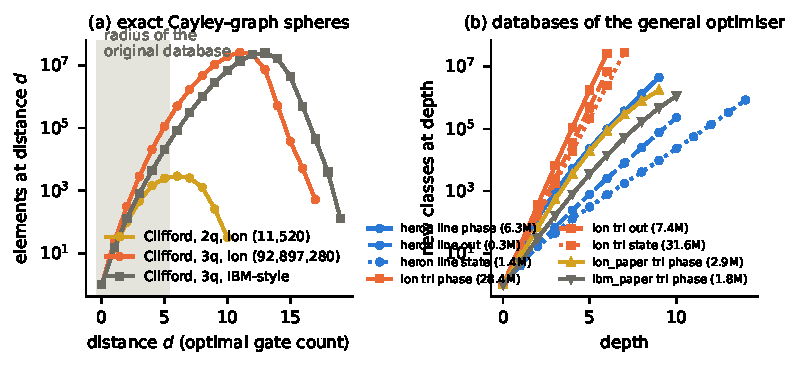
\includegraphics[width=\textwidth]{figs/fig_growth.pdf}
\caption{(a) Sphere sizes $|S(d)|$ of the exact Cayley graphs used as ground truth. The shaded band is the database radius
of~\cite{rosenhahn2025}. The Clifford+T spheres keep growing, since that group is infinite. (b) New classes per depth in the
general optimiser's databases (equality up to phase, one curve per device and alphabet, total size in
parentheses).}\label{fig:growth}
\end{figure}

\subsection{Beyond Clifford: exact two-qubit Clifford+T distances}\label{sec:cliffordt}

With angles in $\{\pm\frac\pi4,\pm\frac\pi2,\pi\}$ the ion alphabet ($\RX,\RY,\RZ$ on each qubit and
$\RXX(\pm\frac\pi4,\pm\frac\pi2)$, 34 gates on two qubits) is universal, and the group is infinite. Up to phase every
generator has entries in $\Dw=\mathbb Z[1/\sqrt2,\omega]$, $\omega=e^{i\pi/4}$, e.g.
\begin{equation}\label{eq:ctgens}
\RZ(\tfrac\pi4)\propto\mathrm{diag}(1,\omega),\quad \RX(\theta)\propto H\RZ(\theta)H,\quad
\RXX(\theta)\propto H^{\otimes2}\mathrm{diag}(1,e^{i\theta},e^{i\theta},1)H^{\otimes2},
\end{equation}
and so does every circuit~\cite{giles2013}. We store $U=M/\sqrt2^{\,k}$ exactly, with $M$ over $\Zw$ in the $\mathbb Z$-basis
$1,\omega,\omega^2,\omega^3$.

\begin{lemma}[Exact projective canonical form]\label{lem:canon}
For $U$ over $\Dw$ let $p$ be the first non-zero entry in row-major order and $P(U)_{ij}=U_{ij}\overline{U_p}$. Then $P(U)$ is
over $\Dw$, and $V=e^{i\varphi}U$ for some $\varphi$ if and only if $V$ has the same first non-zero position and
$P(V)=P(U)$. Writing $P(U)=M'/\sqrt2^{\,k'}$ with the smallest $k'\ge0$ for which $M'$ is over $\Zw$ makes $(M',k')$ unique.
\end{lemma}

We hash the canonical forms into 64-bit keys and grow a ball of radius $R=\CTRadius$ (\CTBallSize\ elements, levels
\CTBallLevels, \CTBallMinutes\ minutes). Equality of the numbers of distinct keys and distinct canonical forms certifies that
no collision occurred. For $|U|\le R+R'$ meet in the middle gives the exact distance
\begin{equation}\label{eq:mitm}
|U|=\min_{0\le j\le R'}\Bigl(j+\min_{Y\in S(j)}\bigl|UY^\dagger\bigr|\Bigr),
\end{equation}
which with $R'=\CTRadius-1$ certifies optimal lengths up to \CTCertified\ and a lower bound beyond.

\paragraph{Planted benchmarks.} Long circuits are beyond any certifiable radius, so we plant the optimum. Starting from a core
$c$ with certified $|\ev(c)|=|c|$, we repeatedly pick a window $W$ (up to four gates) and a word $r$ (up to three gates),
compute a geodesic $s$ of $\ev(W)\ev(r)^{-1}$ exactly and replace $W$ by $rs$. Since $\ev(s)\ev(r)=\ev(W)$ the unitary, and
hence the certified optimum $|c|$, is unchanged, while overlapping windows make the planted structure non-local.

%=====================================================================
\section{Experiments}\label{sec:exp}

\paragraph{Metrics.} For a pipeline $P$ and a set $\mathcal C$ of circuits, count ratios are ratios of sums and ESP ratios
are geometric means,
\begin{equation}\label{eq:ratios}
\rho_{\#}(P)=\frac{\sum_{c\in\mathcal C}\#_P(c)}{\sum_{c\in\mathcal C}\#_{\rm L3}(c)},\qquad
\rho_{\rm ESP}(P)=\Bigl(\prod_{c\in\mathcal C}\frac{\mathrm{ESP}_P(c)}{\mathrm{ESP}_{\rm L3}(c)}\Bigr)^{1/|\mathcal C|},
\end{equation}
relative to Qiskit level 3 (L3) unless stated otherwise.

\paragraph{Verification.} Every output is checked against its input. Exact mode is checked by $\op{(U-V)\psi}$ on random states
(maximum $\IonMaxExactErr$), state-aware mode by the TVD of the output distributions on $|0^n\rangle$ (maximum
$\IonMaxStateErr$), approximate mode against the tracked bound, and Clifford+T outputs by exact equality over $\Dw$. Every
output is also checked to be native and to use only coupled pairs. All \PaperBenchN\ benchmark outputs, all 720
hardware-suite outputs and all Clifford+T and layout outputs pass. BQSKit outputs are checked the same way, up to global phase
and its final qubit permutation. Large-suite outputs are checked by replay certificates, and up to 24 active qubits also by
statevector. Logical-level outputs of every tool are checked up to global phase, by statevector up to 20 qubits and
by~\cite{qcec} above.

\subsection{Discrete benchmarks against ground truth}

We run the general optimiser with the semantics of~\cite{rosenhahn2025} (up to phase, gate count, $\pm\frac\pi2$
alphabets, all-to-all) on their settings and seeds, Tables~III/IV (3 qubits, 300 gates, 20 circuits each), the journal
4-qubit statistics (100 circuits) and Table~V (15 qubits, 500 gates, 10 circuits). ``Original'' is the database method (V2)
of~\cite{rosenhahn2025}, run from the authors' released code ported to Python.

\begin{table}[t]
\caption{Mean gate counts on the discrete benchmarks. $^*$Original and Qiskit at 4 qubits use the first 30 circuits. Cliff.\
CW uses adaptive convex windows with the exact Clifford tables (Appendix~\ref{app:cliff}), which the general optimiser does not
use. Optimum is the proven optimum or a certified lower bound, and \#opt.\ counts circuits on which the general optimiser is
optimal. All \PaperBenchOk/\PaperBenchN\ outputs verified and native.}\label{tab:paperbench}
\small
\begin{tabular*}{\textwidth}{@{\extracolsep\fill}lcccccc}
\toprule
setting & Qiskit & orig. & Cliff.\ CW & general & optimum & \#opt.\\
\midrule
T3, ion, 3q & \QThreeIon & \TThreePaper & -- & \TThreeGen & \TThreeOpt & \TThreeAtOpt/20\\
T4, IBM-style, 3q & \QThreeIbm & \TFourPaper & -- & \TFourGen & \TFourOpt & \TFourAtOpt/20\\
journal, ion, 4q & \QFourIon$^*$ & \NjpIonPaper$^*$ & \NjpIonCliff & \NjpIonGen & $\ge$\LBFourIon & --\\
journal, IBM-style, 4q & \QFourIbm$^*$ & \NjpIbmPaper$^*$ & \NjpIbmCliff & \NjpIbmGen & $\ge$\LBFourIbm & --\\
T5, IBM-style, 15q & \TFiveLThree & \TFivePaper & \TFiveCliff & \TFiveGen & -- & --\\
\botrule
\end{tabular*}
\end{table}

\begin{figure}[t]
\centering
\begin{minipage}{\textwidth}\small
(a) original method, \ExPaperOrig\ gates\par\smallskip
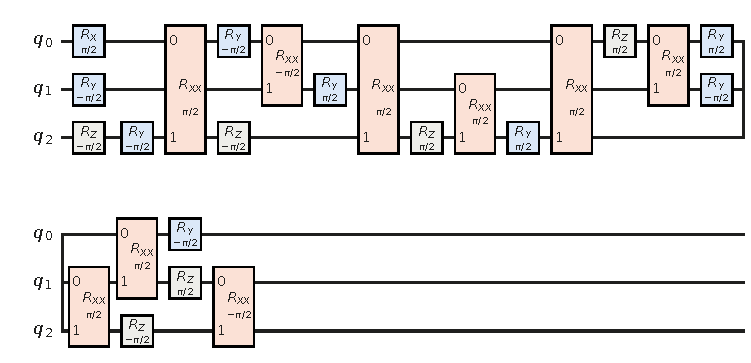
\includegraphics[scale=\cs]{figs/fig_ex_paper_orig.pdf}\par\medskip
(b) proven optimum from the exact Cayley table, \ExPaperOpt\ gates\par\smallskip
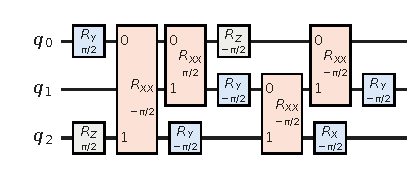
\includegraphics[scale=\cs]{figs/fig_ex_paper_opt.pdf}
\end{minipage}
\caption{One random 3-qubit word of \ExPaperIn\ gates over $\Gamma_{\rm ion}$, after the original method (a) and at its
proven optimum (b). Both panels are drawn at the same scale.}\label{fig:expaper}
\end{figure}

\begin{figure}[t]
\centering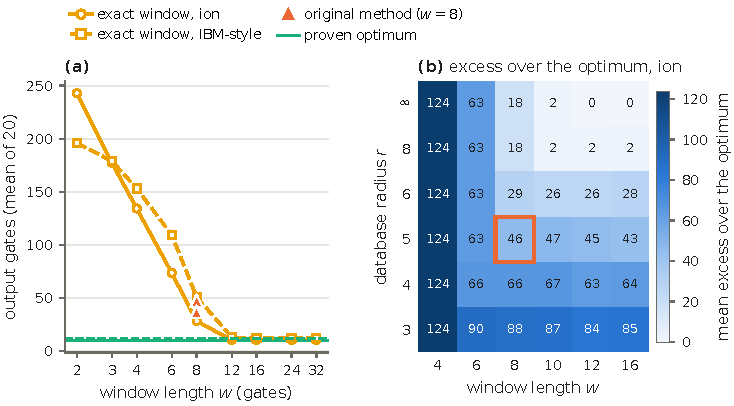
\includegraphics[width=\textwidth]{figs/fig_window_grid.pdf}
\caption{Where the gap to the optimum comes from (3 qubits, exact Clifford tables). (a) Fixed-point length of the exact-window
optimiser against the window length $w$, with the cascade near $w^\star$ of~\eqref{eq:wstar}. (b) Mean excess over the
optimum by window $w$ and database radius $r$ (ion), with the operating point $(8,5)$ of~\cite{rosenhahn2025}
outlined.}\label{fig:window}\label{fig:grid}
\end{figure}

Without knowing that the group is finite or Clifford, the general optimiser is within 0.4 gates of the proven optimum on
average and optimal on 35 of 40 three-qubit circuits, where the original method is $4.5\times$ and $3.0\times$ above it
(Table~\ref{tab:paperbench}, Figs.~\ref{fig:expaper} and~\ref{fig:paperflow}). Fig.~\ref{fig:window} explains the gap. At
$w=8$, raising $r$ from 5 to $\infty$ lowers the mean excess from 46 to 18 gates, enlarging $w$ at $r=5$ barely helps, and
for $w\ge12$, $r\ge8$ the excess is at most 2, as Theorem~\ref{thm:exact} predicts. At four qubits the general optimiser
matches the Clifford-specific one, so large databases and convex windows, not knowledge of the group, make the difference.
At 15 qubits all methods, Qiskit included, lie within 4\% of one another.

\subsection{Certified Clifford+T benchmarks}

On the two-qubit Clifford+T alphabet we compare the general optimiser (ion database over exactly this alphabet), the original
method (compute graph of depth 4 over the same alphabet) and Qiskit level 3 (continuous angles, shown for reference) with the
certified optimum.

\begin{figure}[t]
\centering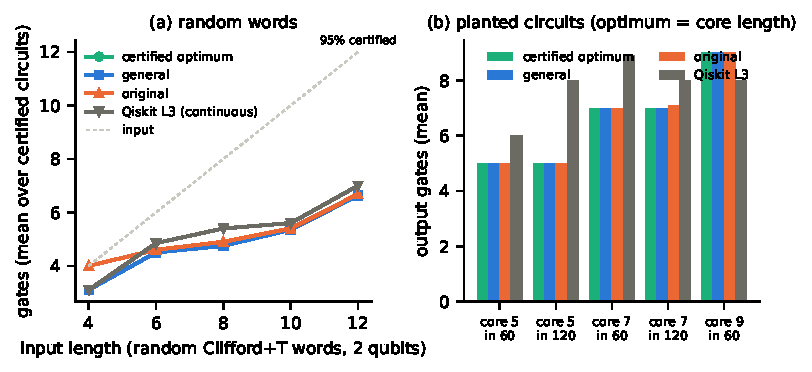
\includegraphics[width=\textwidth]{figs/fig_cliffordt.pdf}
\caption{Clifford+T, two qubits. (a) Random words, mean output length over circuits whose optimum is certified. (b) Planted
circuits, a core of the stated length hidden in 60 or 120 gates.}\label{fig:ct}
\end{figure}

On random words with certified optimum the general optimiser is optimal on \CTRandGenAtOpt\ circuits and the original method
on \CTRandOrigAtOpt\ (Fig.~\ref{fig:ct}). On \CTPlantN\ planted circuits (mean input \CTPlantInputMean, mean optimum
\CTPlantOptMean) the general optimiser reaches the optimum on \CTPlantGenAtOpt/\CTPlantN\ (mean \CTPlantGenMean), the
original method on \CTPlantOrigAtOpt/\CTPlantN\ (mean \CTPlantOrigMean), and Qiskit returns \CTPlantQiskitMean\ gates in its
continuous alphabet. All discrete outputs are exactly equal to their inputs over $\Dw$ (example in Fig.~\ref{fig:exct}).

\subsection{Algorithms on hardware models}

\paragraph{Suite.} \HwCircuits\ circuits of 2--\HeronMaxQubits\ qubits and up to \HeronMaxInput\ gates from Nam/VOQC
arithmetic~\cite{nam2018}, QASMBench~\cite{qasmbench} (without feed-forward), QFT, QAOA, Heisenberg Trotter steps,
EfficientSU2, a Steane encoder and random circuits are compiled by Qiskit at levels 1 and 3 with the same coupling map and
seed. TKET \texttt{FullPeepholeOptimise} and BQSKit~\cite{bqskit} (version 1.2.1, levels 2 and 3, blocks of up to three
qubits resynthesised to $10^{-8}$) start from the level-1 output.

\begin{table}[t]
\caption{Ratios~\eqref{eq:ratios} relative to Qiskit level 3 (\HwCompared\ circuits per device). BQSKit outputs are
approximate. The last row applies our optimiser to a separate BQSKit level-3 run. Nam pf1\_10/pf2\_10 are excluded because
Qiskit level 3 drops their $\sim10^{-7}$\,rad rotations.}\label{tab:hw}
\small\setlength{\tabcolsep}{3pt}
\begin{tabular*}{\textwidth}{@{\extracolsep\fill}lccc c ccc}
\toprule
& \multicolumn{3}{c}{IBM Heron} && \multicolumn{3}{c}{trapped ion}\\\cmidrule{2-4}\cmidrule{6-8}
pipeline & 2q & all & ESP && 2q & all & ESP\\
\midrule
\HwRows
\botrule
\end{tabular*}
\end{table}

\paragraph{Results.} Stacked on level 3 the optimiser never adds a two-qubit gate (\HeronFromLThreeBetter\ circuits better and
\HeronFromLThreeEqual\ equal on Heron, \IonFromLThreeBetter\ and \IonFromLThreeEqual\ on ions) and never lowers ESP
(Table~\ref{tab:hw}, Fig.~\ref{fig:hwflow}, examples in Figs.~\ref{fig:exheron} and~\ref{fig:exheron2}). On Heron it removes
13\% of all gates, mostly $\SX/X$ pulses and virtual $\RZ$. On ions the total can rise (\IonFromLThreeTotalUp\ circuits)
because $c_{\rm cal}$ trades pulses for virtual $\RZ$. From level 1 it beats level 3 on Heron in all gates and, for seed 0, in
ESP, of which $\times$\HeronEspLOneOverLThree\ is due to Qiskit's level-1 layout. State-aware rewriting gives the largest
reductions but empties \HeronStateEmpty\ (Heron) and \IonStateEmpty\ (ion) reversible circuits with a fixed output. The median
run time is \HeronMedianSec\,s (Heron) and \IonMedianSec\,s (ion) per circuit.

\paragraph{Robustness.} Over \SeedN\ transpiler seeds (\SeedOutputs\ verified outputs) the Heron ratios on level 3 are
$\times$\SeedHeronLThreeTwoqMean\ $\pm$ \SeedHeronLThreeTwoqSd\ (two-qubit) and $\times$\SeedHeronLThreeAllMean\ $\pm$
\SeedHeronLThreeAllSd\ (all). From level 1 the gate ratio is equally stable ($\times$\SeedHeronLOneAllMean\ $\pm$
\SeedHeronLOneAllSd), but the ESP gain ranges from $\times$\SeedHeronLOneEspMin\ to $\times$\SeedHeronLOneEspMax\ (mean
$\times$\SeedHeronLOneEspMean), following Qiskit's layout. Optimiser seeds change the total by at most
\SeedHeronOptSpread.

\paragraph{Resynthesis.} From the same level-1 input BQSKit level 3 uses fewer two-qubit gates than ours on
\HeronBqFewerTwoqThanOursLOne\ of \HwCompared\ Heron circuits (more on \HeronBqMoreTwoqThanOursLOne) at about the same ESP,
but \HeronBqAllOverOurs\ times as many gates as ours on level 3, with errors of median $\HeronBqMedErr$ (maximum
$\HeronBqMaxErr$), in \HeronBqMeanSec\,s per circuit on eight workers against \HeronOursMeanSec\,s on one. The two combine. On
a BQSKit level-3 output (\HeronStackInTwoq\ two-qubit and \HeronStackInAll\ total gates on Heron) our optimiser reduces the
total to \HeronStackAll\ ($\times$\HeronStackAllOverBq), never adds a two-qubit gate and raises ESP on \HeronStackEspUp\
circuits ($\times$\HeronStackEspOverBq), in \HeronStackMeanSec\,s per circuit. On ions BQSKit's output is already lean
($\times$\IonStackAllOverBq).

\subsection{What each component contributes}\label{sec:ablation}

\begin{table}[t]
\caption{Ablation on the hardware suite (\AblationCircuits\ circuits per device, seed 0), ratios~\eqref{eq:ratios}
relative to Qiskit level 3. Each row changes one component of the full optimiser. All outputs verified.}\label{tab:ablation}
\footnotesize
\begin{tabular*}{\textwidth}{@{\extracolsep\fill}lccc c cc c cc}
\toprule
& \multicolumn{3}{c}{Heron, from L3} && \multicolumn{2}{c}{Heron, from L1} && \multicolumn{2}{c}{ion, from L1}\\
\cmidrule{2-4}\cmidrule{6-7}\cmidrule{9-10}
variant & saved & 2q & ESP && all & 2q && all & 2q\\
\midrule
\AblationRows
\botrule
\end{tabular*}
\end{table}

On Heron from level 3 the full optimiser saves \AblationFullSaved\ of all gates (Table~\ref{tab:ablation}). The window length
matters most ($w=8$ gives \AblationWEightSaved, $w=4$ gives \AblationWFourSaved), then the database (none
\AblationNoDbSaved, radius 3 \AblationRadiusThreeSaved), the same two parameters that set the gap in Fig.~\ref{fig:window}.
Analytic resynthesis gives most of the rest (\AblationNoResynthSaved\ without it) and reduces the M{\o}lmer--S{\o}rensen
count on ions (\AblationIonNoResynthTwoq\ of level 3's two-qubit gates without it, \AblationIonFullTwoq\ with it). Convex
windows and shuffles add a little each and meet in the middle almost nothing (\AblationNoMitmSaved). Counting gates instead
of $c_{\rm cal}$ saves as many gates but raises ESP only by \AblationHeronCountEsp\ instead of \AblationHeronCalEsp.

\subsection{Large circuits}\label{sec:large}

\LargeCircuits\ Nam/VOQC circuits~\cite{nam2018} of 14 to 100 qubits are compiled by Qiskit for the 133-qubit Heron model and
an all-to-all ion model. Product-formula circuits (\LargeHeronPfN\ per device) are excluded as in Table~\ref{tab:hw}, and so are
circuits with an unchecked certificate (\LargeHeronPending\ Heron, \LargeIonPending\ ion), leaving \LargeHeronN\ Heron circuits
of \LargeHeronMinQubits--\LargeHeronMaxQubits\ qubits and \LargeIonN\ ion circuits with up to \LargeHeronMaxInput\ input
gates. BQSKit ran on the \LargeBqCircuits\ smallest circuits before it was stopped for time.

\begin{table}[t]
\caption{Large circuits, ratios~\eqref{eq:ratios} relative to Qiskit level 3 (\LargeHeronN\ Heron and \LargeIonN\ ion
circuits of up to \LargeHeronMaxQubits\ qubits). ESP ratios are over the \LargeHeronEspN\ Heron and \LargeIonEspN\ ion
circuits with level-3 ESP at least $\LargeEspMin$, below which ESP is dominated by noise. Every output of our optimiser has an
accepted replay certificate.}\label{tab:large}
\begin{tabular*}{\textwidth}{@{\extracolsep\fill}lccc c ccc}
\toprule
& \multicolumn{3}{c}{IBM Heron} && \multicolumn{3}{c}{trapped ion}\\\cmidrule{2-4}\cmidrule{6-8}
pipeline & 2q & all & ESP && 2q & all & ESP\\
\midrule
\LargeRows
\botrule
\end{tabular*}
\end{table}

Stacked on level 3 the optimiser removes \LargeHeronFromLThreeAllSaved\ of all gates and \LargeHeronFromLThreeTwoqSaved\ of
the two-qubit gates on Heron, removes two-qubit gates on \LargeHeronFromLThreeBetter\ of \LargeHeronN\ circuits, never adds one,
and raises ESP by $\times$\LargeHeronFromLThreeEsp\ (median $\times$\LargeHeronFromLThreeEspMedAll\ over all \LargeHeronN), with
the same guarantees on ions (Table~\ref{tab:large}). From level 1 it ends with fewer gates than level 3 on every Heron circuit,
but with more two-qubit gates on \LargeHeronLOneTwoqMore\ and lower ESP, since at this scale layout and routing dominate. On
ions it uses fewer two-qubit gates than level 3 on \LargeIonLOneTwoqFewer\ circuits and more on none. On the \LargeBqHeronN\
circuits BQSKit completed (up to \LargeBqHeronMaxQubits\ qubits) BQSKit level 3 has \LargeHeronBqLThreeTwoq\ two-qubit gates
on Heron against our \LargeHeronOursLThreeTwoq, but \LargeHeronBqLThreeAll\ gates in total against \LargeHeronOursLThreeAll\
(ions \LargeIonBqLThreeTwoq/\LargeIonBqLThreeAll\ against \LargeIonOursLOneTwoq/\LargeIonOursLOneAll), with errors up to
$\LargeBqMaxErr$ on at most 24 qubits and \LargeBqUnchecked\ wider outputs unchecked.

\paragraph{Certificates and run time.} \LargeCertOk\ of \LargeOutputs\ outputs have an accepted certificate
(Proposition~\ref{prop:cert}), each with up to \LargeCertMaxSteps\ steps, at most \LargeCertMaxSec\,s to check and residuals
below $\LargeCertMaxErr$. A first checker rejected \LargeCertFirstRejected\ certificates because it checked the phase repair
as one block beyond its 12-wire limit. The current checker checks each patch separately and accepted all
\LargeCertRechecked\ re-run cases, and \LargeCertPending\ were not re-checked. Median run times (Table~\ref{tab:runtime}) are
seconds per circuit on the 60-circuit suite and minutes, up to \LargeHeronMaxSec\,h, on the large suite in single-threaded
Python, the main cost of the method at scale.

\subsection{Logical-level comparison}\label{sec:logical}

Quartz~\cite{quartz}, QUESO~\cite{queso} and VOQC~\cite{voqc} are evaluated on the Nam gate set $\{H,X,\RZ,\CNOT\}$,
all-to-all, with total gate count as objective, on \LogicalCircuits\ arithmetic and Toffoli circuits of~\cite{nam2018}. Our
optimiser runs unchanged with a database over this gate set and equality up to phase. Every tool starts from the decompositions
distributed with QUESO. VOQC runs its full Nam pass sequence and QUESO its recommended rule sets with five minutes per circuit
(one hour on \LogicalQuesoHourN\ small circuits improves its total from \LogicalQuesoFiveOnHourTotal\ to
\LogicalQuesoHourTotal). All \LogicalOutputs\ outputs are equal to their inputs up to phase.

\begin{table}[t]
\caption{Logical level, Nam gate set, summed over \LogicalCircuits\ circuits, changes relative to the input. The last column
counts circuits on which a tool is best or tied among the single tools. All outputs verified.}\label{tab:logical}
\small
\begin{tabular*}{\textwidth}{@{\extracolsep\fill}lccccc}
\toprule
tool & gates & change & CNOT & change & best on\\
\midrule
\LogicalRows
\botrule
\end{tabular*}
\end{table}

VOQC removes \LogicalVoqcSaved\ of the gates and is best on most circuits, and ours removes \LogicalOursSaved, ahead of QUESO,
Qiskit and TKET (Table~\ref{tab:logical}). VOQC merges rotations over phase polynomials arbitrarily far apart, while our windows
see three qubits, and our windows find rewrites VOQC does not (\texttt{mod5\_4}, \LogicalModFiveOurs\ against
\LogicalModFiveVoqc\ gates). Run on VOQC's output, our optimiser improves \LogicalVoqcOursBeatsVoqc\ of \LogicalCircuits\
circuits and gives the best result overall, \LogicalVoqcOursSaved\ fewer gates and \LogicalVoqcOursCxSaved\ fewer CNOTs than
the input. Quartz was not run.

\subsection{Real hardware}\label{sec:realhw}

\begin{definition}[Hardware metric]\label{def:hwmetric}
For a circuit $c$ with deterministic ideal output $x^\star$, a pipeline $P$ and job $j$, let $\hat p_{P,j}(c)$ be the fraction of
shots returning $x^\star$, and $\bar p_P(c)$ its mean over jobs. The summary over $N$ circuits is
\begin{equation}\label{eq:hwratio}
\rho_{\rm hw}(P)=\Bigl(\prod_{c}\frac{\bar p_P(c)}{\bar p_{\rm L3}(c)}\Bigr)^{1/N},
\end{equation}
and per circuit we report the mean and standard deviation over $j$ of the paired ratio $\hat p_{P,j}(c)/\hat p_{{\rm L3},j}(c)$,
whose two factors share one calibration.
\end{definition}

We ran $N=\HwRealN$ circuits of \HwRealMinQ--\HwRealMaxQ\ qubits on \HwRealBackend\ (IBM Heron r2), compiled by level 3, by
level 3 followed by our optimiser and by level 1 followed by our optimiser, in \HwRealRepeats\ jobs of \HwRealShots\ shots with
the circuit order shuffled per job. Our optimiser on level 3 gives $\rho_{\rm hw}=\HwRealLThreeRatio$ (better on
\HwRealLThreeWins/\HwRealN) and on level 1 \HwRealLOneRatio\ (\HwRealLOneWins/\HwRealN), against \HwDryLThreeRatio\ predicted by
the noise model (Fig.~\ref{fig:hwreal}). On these circuits it removes \HwRealAllSaved\ of the gates but two-qubit gates on only
\HwRealTwoqFewerN, and the effect is below the spread between jobs.

\begin{figure}[t]
\centering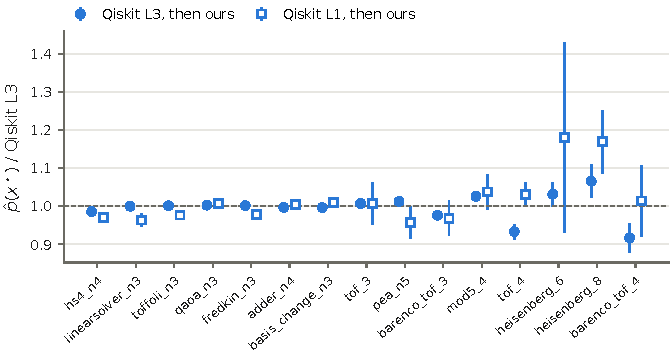
\includegraphics[width=\textwidth]{figs/fig_hw_real.pdf}
\caption{\HwRealBackend, paired ratio of Definition~\ref{def:hwmetric} relative to Qiskit level 3, mean and one standard
deviation over \HwRealRepeats\ jobs. Circuits are sorted by level-3 gate count.}\label{fig:hwreal}
\end{figure}

\subsection{Choosing the objective}

We ran the optimiser with each cost of~\eqref{eq:costs} and computed the exact TVD between ideal and noisy output
distributions from density matrices (Heron calibrated errors of the actual qubits, ion depolarising noise at the model rates)
on the \HeronTvdCircuits\ circuits with at most eight active qubits (Table~\ref{tab:tvd}). The calibrated cost is at least as
good as the alternatives on both devices and beats Qiskit level 3 on \HeronCalBeatsLThree/\HeronTvdCircuits\ Heron circuits.
Where no calibration exists, $c_{w2}$ is a good proxy.

\subsection{Layout-aware rewriting}

On Heron we compare, for \LayN\ circuits, Qiskit level 3 with and without the calibrated target (noise-aware layout), our
optimiser on each, relocation~\eqref{eq:reloc} after the noise-aware pipeline, and joint layout selection over four seeds and
two modes, with readout errors in ESP and in the noisy simulation.

\begin{table}[t]
\caption{Layout-aware rewriting on IBM Heron. ESP~\eqref{eq:esp} includes readout, ratios are geometric means relative to
Qiskit's noise-aware level 3, and TVD is the mean exact noisy TVD including readout (\LayTvdN\ circuits).}\label{tab:layout}
\begin{tabular*}{\textwidth}{@{\extracolsep\fill}lccc}
\toprule
pipeline & ESP ratio & two-qubit gates (sum) & TVD\\
\midrule
Qiskit L3 (coupling map only) & $\times$\LayEspLThree & \LayTwoqLThree & \LayTvdLThree\\
Qiskit L3, noise-aware & $\times$1.00 & \LayTwoqNA & \LayTvdNA\\
noise-aware + \qcr & $\times$\LayEspNAOurs & \LayTwoqNAOurs & \LayTvdNAOurs\\
noise-aware + \qcr\ + relocation & $\times$\LayEspRel & \LayTwoqRel & \LayTvdRel\\
joint layout selection (\qcr) & $\times$\LayEspJoint & \LayTwoqJoint & \LayTvdJoint\\
\botrule
\end{tabular*}
\end{table}

Placement dominates (Table~\ref{tab:layout}, Fig.~\ref{fig:layout}). Qiskit's noise-aware layout raises ESP by $1/$\LayEspLThree\
over the coupling-map-only layout, relocation after rewriting adds $\times$\LayEspRel\ and joint selection $\times$\LayEspJoint,
with lower noisy TVD than the noise-aware baseline on \LayJointBeatsNA/\LayTvdN\ circuits. Joint selection chose a noise-aware
candidate in only \LayJointNAShare\ of the circuits, so the best final layout is often not the one ranked best before
optimisation.

%=====================================================================
\section{Discussion and limitations}\label{sec:discussion}

\paragraph{What the ground truth shows.} For discrete alphabets, local rewriting is rewriting on a Cayley graph, and its
quality is governed by the database radius and the window through Theorem~\ref{thm:exact} and the cascade~\eqref{eq:wstar}.
Large hashed databases and convex windows close almost all of the gap to the optimum without using the group structure.

\paragraph{Exact rewriting and global passes.} Resynthesis (BQSKit) finds cheaper entangling structure inside blocks and
rotation merging (VOQC) combines rotations far apart, both out of reach of stored rewrites on three-qubit windows. Exact local
rewriting is faster, keeps the unitary including phase and removes what these passes leave (\HeronStackAllSaved\ after BQSKit on
Heron, the best of all tools after VOQC). A practical pipeline runs a global pass first and exact local rewriting last.

\paragraph{Limitations.}
(i) \emph{Hardware evidence.} ESP and TVD come from calibration snapshots without idle errors or crosstalk, and the device run
(Section~\ref{sec:realhw}) covers \HwRealN\ small circuits, where the effect is below the run-to-run spread.
(ii) \emph{Global phase.} Exactness including phase costs \HeronPhaseGadgetGates\ single-qubit gates over the Heron suite. With
phase as metadata the all-gate ratio from level 1 would improve from $\times0.838$ to $\times0.825$.
(iii) \emph{Baselines.} Quartz was not run, QUESO had five minutes per circuit instead of one hour, other baselines use default
settings, and on the large suite BQSKit covers only the \LargeBqCircuits\ smallest circuits.
(iv) \emph{Scale.} Windows have at most three qubits, the code is single-threaded Python, and feed-forward is out of scope.
Two 64-qubit Heron runs did not finish and \LargeCertPending\ certificates were not re-checked.
(v) \emph{Ground truth} beyond Clifford is certified for two qubits and lengths up to \CTCertified.
(vi) \emph{Verification} is numerical up to 24 qubits and by replay certificates beyond, and exact only for Clifford and
Clifford+T circuits.

\paragraph{Future work.} A theory of $w^\star$ would relate the cascade to Dehn presentations and local geodesics in
groups~\cite{gromov1987,epstein1992} and to complete rewriting systems~\cite{knuthbendix1970}. Reaching the entangling
structure that resynthesis finds without giving up exactness needs four-qubit databases with symmetry reduction, or
resynthesised blocks with angles snapped to exactly realisable values and then verified. On hardware, the next step is
repeated runs on circuits where rewriting removes two-qubit gates.

%=====================================================================
\section{Conclusion}\label{sec:conclusion}

Making ``equivalent'' precise as a group action turns local rewriting into an exact, hardware-aware optimiser with provable
guarantees. Built without using the structure of any gate set, it reaches proven optima on discrete three-qubit benchmarks and
on planted Clifford+T circuits, improves Qiskit's level-3 output on real algorithms without adding two-qubit gates, scales to
\LargeHeronMaxQubits\ qubits with independently checked certificates, and adds exact savings after BQSKit and VOQC. Exact
ground truth, Clifford and beyond, is what makes such claims checkable.

\FloatBarrier
\backmatter

\bmhead{Acknowledgements}
We thank the authors of~\cite{rosenhahn2025} for publishing their code, and the developers of Qiskit, Qiskit Aer, TKET,
BQSKit, VOQC, QUESO, QASMBench and the VOQC benchmarks.

\section*{Declarations}

\begin{itemize}
\item \textbf{Funding:} No funding was received for this work.
\item \textbf{Competing interests:} The author declares no competing interests.
\item \textbf{Ethics approval and consent to participate:} Not applicable.
\item \textbf{Consent for publication:} Not applicable.
\item \textbf{Data availability:} All raw results, logs and figure data are included in the repository below
  (\texttt{results/}).
\item \textbf{Materials availability:} Not applicable.
\item \textbf{Code availability:} The implementation (\qcr, Apache License 2.0), every experiment script and the scripts that
  generate all tables, figures and numbers in this paper are available at \url{https://github.com/arnavk23/qcr}.
\item \textbf{Author contribution:} A.K.\ conceived the study, developed the software, performed the experiments and wrote
  the manuscript.
\end{itemize}

\bibliography{refs}

\clearpage
\begin{appendices}

\section{Proofs}\label{app:proofs}

\begin{proof}[Proof of Proposition~\ref{prop:sound}]
By convexity, $S$ can be moved to the front (a) or the back (b) of the circuit without changing $\ev(u)$. In case (a) the
input factorises as $|0_W\rangle\otimes|0_{\bar W}\rangle$, so the final state changes only by the global phase
$e^{i\varphi}$. In case (b) the final state changes from $|\psi\rangle$ to $(D\otimes I)|\psi\rangle$, and
$|\langle x|(D\otimes I)|\psi\rangle|^2=|\langle x|\psi\rangle|^2$ for every basis state $x$. Since the invariant is the
output distribution of the current circuit, soundness composes.
\end{proof}

\begin{proof}[Proof of Proposition~\ref{prop:approx}]
Telescope over $u=u_0,u_1,\dots,u_m=u'$. Each step changes one factor of a product of unitaries, $\ev(u_t)=A\,\ev(v_t)\,B$
and $\ev(u_{t-1})=A\,\ev(S_t)\,B$ with unitary $A,B$, and $\op{A(X-Y)B}=\op{X-Y}$.
\end{proof}

\begin{proof}[Proof of Proposition~\ref{prop:cert}]
A swap changes $\ev$ by $A(\gamma'\gamma-\gamma\gamma')B$ with unitary $A,B$, of norm at most $\delta_t$, so we may take
$\lambda_t=1$ for swaps. A replacement gives $\ev(u_t)=A\,\ev(v)\,B=\lambda_t\ev(u_{t-1})+E_t$ with $\op{E_t}\le\delta_t$.
Inductively $\ev(u')=\Lambda\,\ev(u)+E$ with $\Lambda=\prod_t\lambda_t$ and $\op E\le\sum_t\delta_t\prod_{s>t}|\lambda_s|$.
Since $\ev(v)$ and $\ev(s)$ are unitary, $\bigl||\lambda_s|-1\bigr|\le\delta_s$, hence
$\op{\ev(u')-\ev(u)}\le|\Lambda-1|+\op E\le\delta_0+\sum_t\delta_t+O(\delta^2)$.
\end{proof}

\begin{proof}[Proof of Lemma~\ref{lem:clifford}]
All generators map Paulis to Paulis under conjugation, so $\langle\Gamma\rangle\subseteq\Cl_n/U(1)$. The single-qubit
generators generate $\Cl_1$, and an entangling Clifford together with $\Cl_1^{\otimes n}$ generates
$\Cl_n$~\cite{selinger2015}. Enumeration confirms the orders 24, 11,520 and 92,897,280 for $n=1,2,3$.
\end{proof}

\begin{proof}[Proof of Theorem~\ref{thm:exact}]
Let $u$ be $(w,r)$-reduced. If $|u|>D$, its first $D+1$ letters form a factor $f$ with $|\ev(f)|\le D\le r$ and
$|f|=D+1\le w$, so the rule $f\to v$ with $v$ a geodesic of $\ev(f)$ applies, a contradiction. Hence $|u|\le D<w$, so $u$
is itself a factor of length at most $w$. If it were not geodesic, the rule $u\to v$ with $v$ a geodesic of $\ev(u)$ and
$|v|\le D\le r$ would apply.
\end{proof}

\begin{proof}[Proof of Proposition~\ref{prop:cascade}]
If the whole word is a factor of length at most $w$ and the database has unbounded radius, the word itself is replaced by
a geodesic of its value. A fixed point of length $\ell(w)\le w$ is therefore a geodesic, and $w^\star$ is the smallest
window for which this happens.
\end{proof}

\begin{proof}[Proof of Theorem~\ref{thm:parity}]
A Cayley graph is bipartite if and only if there is a homomorphism $\chi:G\to\{\pm1\}$ with $\chi(\Gamma)=-1$. (a) For
$n=1$, $\Cl_1/U(1)\cong S_4$ and every $\pm\frac\pi2$ rotation is a 4-cycle, so $\chi=\mathrm{sgn}$ works. For $n=2$ we
verify bipartiteness exhaustively (no edge joins two elements at equal distance from the identity). (b) The Pauli group
$\mathcal P_n$ is normal with quotient $\Sp(2n,2)$. If $\chi$ existed, then $\chi(X_i)=\chi(\gamma)^2=1$ and likewise
$\chi(Z_i)=1$, so $\chi$ would factor through $\Sp(2n,2)$, which is simple and non-abelian for $n\ge3$. Hence
$\chi\equiv1$, contradicting $\chi(\Gamma)=-1$.
\end{proof}

\begin{proof}[Proof of Theorem~\ref{thm:mix}]
This is the standard $L^2$ bound for random walks on groups~\cite{diaconis1988}. By Cauchy--Schwarz,
$\|\mu_L-\pi_L\|_{TV}\le\frac12\sqrt{|G|}\,\|\mu_L-\pi_L\|_2$, and the walk operator contracts the component orthogonal to
the constants (and, in the bipartite case, to the sign character) by at least $\beta$ per step. The limit of the expected
length follows because $|\ev(u)|\le D$.
\end{proof}

\begin{proof}[Proof of Proposition~\ref{prop:count}]
A geodesic of length $a+b$ splits into geodesics of lengths $a$ and $b$, so $S(a+b)\subseteq S(a)S(b)$. Bounding $|B(d)|$
from above by these products bounds $\Pr[|g|\le d]$ from above, and $\mathbb E|g|=\sum_{d\ge0}\Pr[|g|>d]$.
\end{proof}

\begin{proof}[Proof of Lemma~\ref{lem:canon}]
$\Dw$ is closed under products and conjugation ($\overline\omega=-\omega^3$). If $V=e^{i\varphi}U$, the zero patterns agree
and $V_{ij}\overline{V_p}=U_{ij}\overline{U_p}$. Conversely, $P(V)=P(U)$ at $(i,j)=p$ gives $|V_p|=|U_p|$, so
$V_p=e^{i\varphi}U_p$ for some $\varphi$, and then $V_{ij}=U_{ij}\overline{U_p}/\overline{V_p}=e^{i\varphi}U_{ij}$.
Uniqueness holds because $1,\omega,\omega^2,\omega^3$ is a $\mathbb Z$-basis of $\Zw$ and the smallest common exponent is
unique. Divisibility by $\sqrt2=\omega-\omega^3$ is decided exactly by checking that all coefficients of $M\sqrt2$ are even.
\end{proof}

\FloatBarrier
\section{Clifford-specific optimisers}\label{app:cliff}

For the alphabets of Section~\ref{sec:theory} the exact tables give an \emph{exact-window} optimiser EW-$w$, which replaces
every window of length at most $w$ on at most three wires by an optimal word, and its convex version CW-$w$. CW-sem grows
windows adaptively while gates commute into them.

\begin{table}[!htbp]
\caption{Mean gate counts on the 3-qubit benchmarks (300 gates, 20 circuits).}\label{tab:gap}
\begin{tabular*}{\textwidth}{@{\extracolsep\fill}lccccc}
\toprule
& optimum & original & EW-8 & EW-16 & Qiskit L3\\
\midrule
ion & \OptIon & \FaithIon & \EWeightIon & \EWsixteenIon & \QThreeIon\\
IBM-style & \OptIbm & \FaithIbm & \EWeightIbm & \EWsixteenIbm & \QThreeIbm\\
time per circuit (ion) & -- & \FaithIonSec\,s & \EWeightIonSec\,s & \EWsixteenIonSec\,s & $<$0.1\,s\\
\botrule
\end{tabular*}
\end{table}

\GapFindings

\begin{table}[!htbp]
\caption{4-qubit benchmark (300 gates, 100 circuits). Original (orig.) and Qiskit level 3 use the first 30 circuits.
Published (publ.) numbers are from the journal version of~\cite{rosenhahn2025}. BQSKit level 4 is our run on the first
\BqFourN\ circuits, with the same gate set at continuous angles (approximate, all-to-all).}\label{tab:four}
\small\setlength{\tabcolsep}{3pt}
\begin{tabular*}{\textwidth}{@{\extracolsep\fill}lcccccccc}
\toprule
& bound & CW-sem & CW-24 & EW-16 & orig. & publ. & Qiskit & BQSKit\\
\midrule
ion, total & $\ge$\LBFourIon & \NjpIonCliff & \CWFourIon & \EWFourIon & \FaithFourIon & 111 & \QFourIon & \BqFourIon\\
ion, $\RXX$ & -- & -- & \CWFourIonTwoQ & \EWFourIonTwoQ & \FaithFourIonTwoQ & 43 & \QFourIonTwoQ & \BqFourIonTwoQ\\
IBM-style, total & $\ge$\LBFourIbm & \NjpIbmCliff & \CWFourIbm & \EWFourIbm & \FaithFourIbm & 107 & \QFourIbm & \BqFourIbm\\
IBM-style, $\CZ$ & -- & -- & \CWFourIbmTwoQ & \EWFourIbmTwoQ & \FaithFourIbmTwoQ & 43 & \QFourIbmTwoQ & \BqFourIbmTwoQ\\
\botrule
\end{tabular*}
\end{table}

\FourFindings

\FloatBarrier
\section{Additional figures and tables}\label{app:extra}

\begin{table}[!htbp]
\caption{Median run time per circuit in seconds. Qiskit level 1 was not timed on the 60-circuit suite. On the large suite
BQSKit covers only the \LargeBqCircuits\ smallest circuits, and part of its run shared the machine with an unrelated job. The
large suite ran several circuits at a time on eight cores.}\label{tab:runtime}
\begin{tabular*}{\textwidth}{@{\extracolsep\fill}lcc c cc}
\toprule
& \multicolumn{2}{c}{60-circuit suite} && \multicolumn{2}{c}{large suite}\\\cmidrule{2-3}\cmidrule{5-6}
pipeline & Heron & ion && Heron & ion\\
\midrule
\RuntimeRows
\botrule
\end{tabular*}
\end{table}

\begin{table}[!htbp]
\caption{Mean noisy-simulation TVD by objective (lower is better).}\label{tab:tvd}
\begin{tabular*}{\textwidth}{@{\extracolsep\fill}lccccc}
\toprule
& Qiskit L1 & Qiskit L3 & ours, $c_{\rm count}$ & ours, $c_{w2}$ & ours, $c_{\rm cal}$\\
\midrule
Heron & \HeronTvdLOne & \HeronTvdLThree & \HeronTvdCount & \HeronTvdWTwo & \HeronTvdCal\\
ion & \IonTvdLOne & \IonTvdLThree & \IonTvdCount & \IonTvdWTwo & \IonTvdCal\\
\botrule
\end{tabular*}
\end{table}

\begin{table}[!htbp]
\caption{Hashed databases of the general optimiser (classes per equivalence notion).}\label{tab:dbs}
\begin{tabular*}{\textwidth}{@{\extracolsep\fill}lllrrr}
\toprule
device & topology & notion & depth & classes & build time\\
\midrule
Heron & line & up to phase & 9 & 6.31M & 6 min\\
Heron & line & output-aware & 10 & 0.34M & $<$1 min\\
Heron & line & input-aware & 14 & 1.41M & $<$1 min\\
ion & triangle & up to phase & 6 & 28.4M & 38 min\\
ion & triangle & output-aware & 6 & 7.36M & 27 min\\
ion & triangle & input-aware & 7 & 31.6M & 23 min\\
ion ($\pm\frac\pi2$) & triangle & up to phase & 9 & 2.93M & 7 min\\
IBM ($\pm\frac\pi2$) & triangle & up to phase & 10 & 1.84M & 2 min\\
\botrule
\end{tabular*}
\end{table}

\begin{figure}[!htbp]
\centering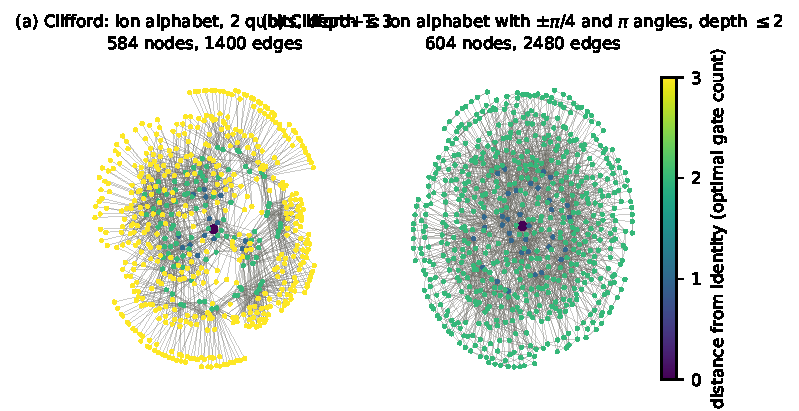
\includegraphics[width=\textwidth]{figs/fig_compute_graph.pdf}
\caption{Compute graphs of comparable size, nodes coloured by exact distance from the identity. (a) Two-qubit Clifford
group, ion alphabet. Many short words coincide and the ball closes up. (b) Two-qubit Clifford+T. Almost every word is
new.}\label{fig:cg}
\end{figure}

\begin{figure}[!htbp]
\centering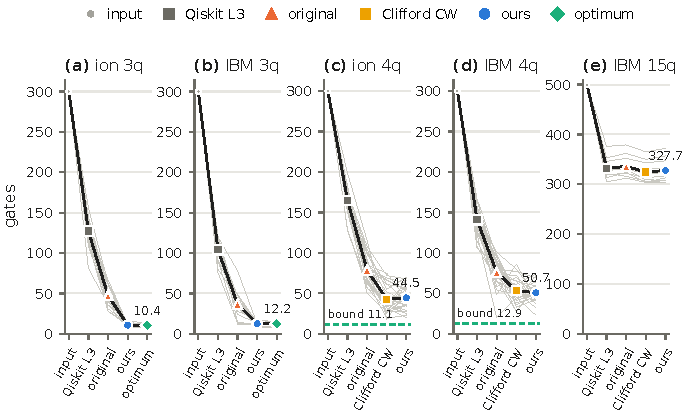
\includegraphics[width=\textwidth]{figs/fig_paper_flow.pdf}
\caption{From the input to the output of every method on the discrete benchmarks. Grey lines are individual circuits (paired
by seed), the black line is the mean and the number is the final mean. The dashed line at 4 qubits is the certified lower
bound of Proposition~\ref{prop:count}.}\label{fig:paperflow}
\end{figure}

\begin{figure}[!htbp]
\centering
\begin{minipage}{\textwidth}\small
(a) planted Clifford+T circuit, \ExCtIn\ gates\par\smallskip
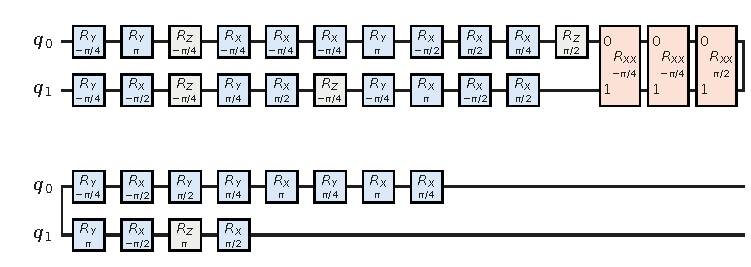
\includegraphics[scale=\cs]{figs/fig_ex_ct_input.pdf}\par\medskip
(b) general optimiser, \ExCtOut\ gates (certified optimum \ExCtOpt)\par\smallskip
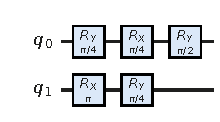
\includegraphics[scale=\cs]{figs/fig_ex_ct_out.pdf}
\end{minipage}
\caption{A planted Clifford+T circuit and the output of the general optimiser, exactly equal over $\Dw$.}\label{fig:exct}
\end{figure}

\begin{figure}[!htbp]
\centering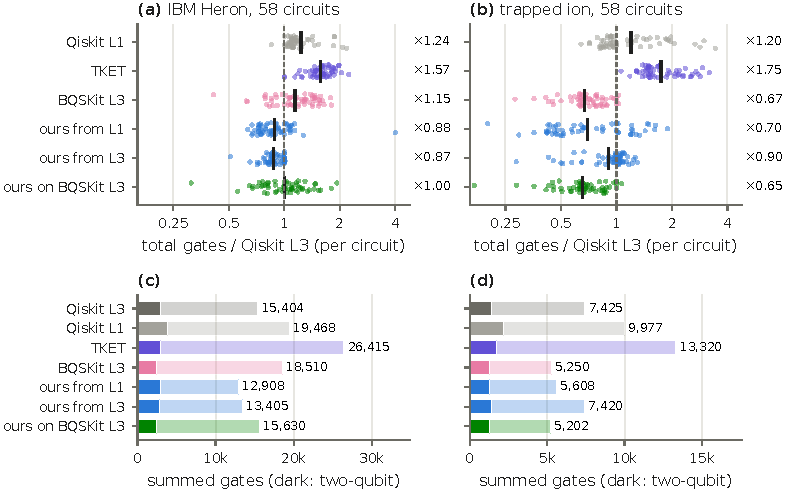
\includegraphics[width=\textwidth]{figs/fig_hw_flow.pdf}
\caption{Hardware suite. (a, b) Total gates per circuit relative to Qiskit level 3 (dots) and geometric means (bars and
labels). (c, d) Summed gates over all circuits, two-qubit gates dark.}\label{fig:hwflow}
\end{figure}

\begin{figure}[!htbp]
\centering
\begin{minipage}{\textwidth}\small
(a) after Qiskit level 3, \ExTofLThree\ gates, \ExTofLThreeCz\ $\CZ$\par\smallskip
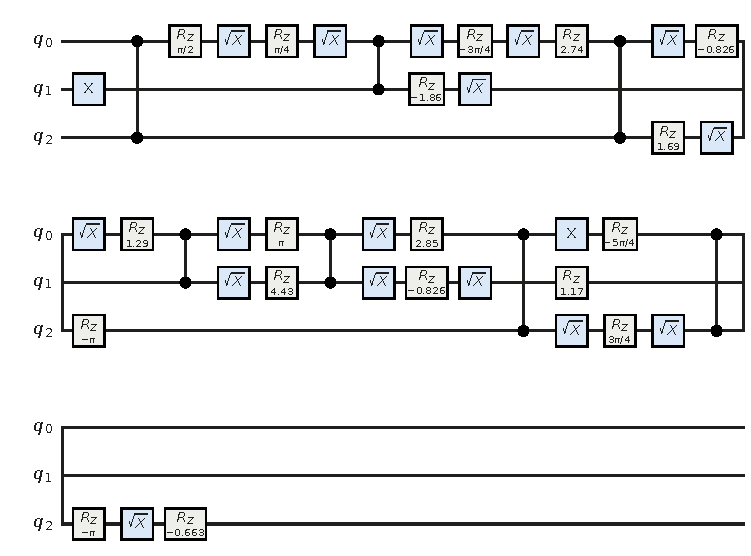
\includegraphics[scale=\cs]{figs/fig_ex_toffoli_n3_l3.pdf}\par\medskip
(b) after \qcr, \ExTofOurs\ gates, \ExTofOursCz\ $\CZ$\par\smallskip
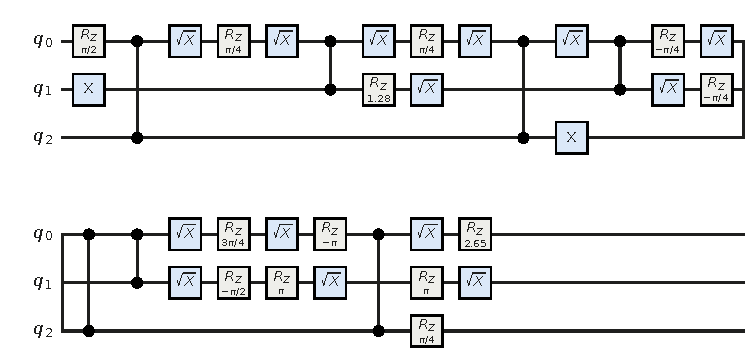
\includegraphics[scale=\cs]{figs/fig_ex_toffoli_n3_ours.pdf}
\end{minipage}
\caption{QASMBench \texttt{toffoli\_n3} on IBM Heron. The outputs are equal including global phase. Blue boxes are pulsed
gates and grey boxes virtual $\RZ$.}\label{fig:exheron}
\end{figure}

\begin{figure}[!htbp]
\centering
\begin{minipage}{\textwidth}\small
(a) after Qiskit level 3, \ExHsLThree\ gates, \ExHsLThreeCz\ $\CZ$\par\smallskip
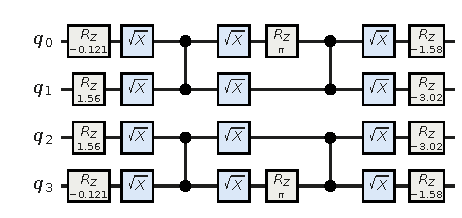
\includegraphics[scale=\cs]{figs/fig_ex_hs4_n4_l3.pdf}\par\medskip
(b) after \qcr, \ExHsOurs\ gates, \ExHsOursCz\ $\CZ$\par\smallskip
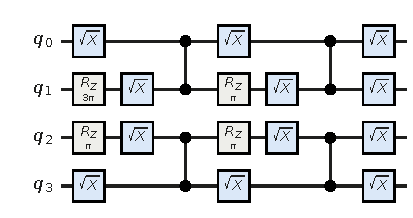
\includegraphics[scale=\cs]{figs/fig_ex_hs4_n4_ours.pdf}
\end{minipage}
\caption{QASMBench \texttt{hs4\_n4} on IBM Heron, drawn as in Fig.~\ref{fig:exheron}.}\label{fig:exheron2}
\end{figure}

\begin{figure}[!htbp]
\centering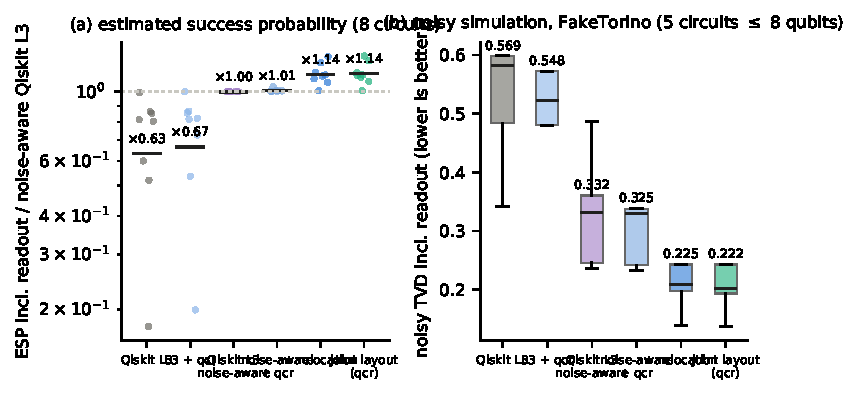
\includegraphics[width=\textwidth]{figs/fig_layout.pdf}
\caption{Layout-aware rewriting on IBM Heron (FakeTorino). (a) ESP including readout relative to Qiskit's noise-aware level
3 (dots are circuits, bars and labels geometric means). (b) Exact noisy TVD including readout for circuits with at most
eight active qubits (bars and labels are means).}\label{fig:layout}
\end{figure}

\FloatBarrier
\end{appendices}

\end{document}
